\documentclass{article}
\usepackage[utf8]{inputenc}
\usepackage{amsmath}
\usepackage{amssymb}
\usepackage{amsthm}
\usepackage{geometry}
\usepackage{graphicx}
\usepackage{float}
\usepackage{listings}
\usepackage{xcolor}
\usepackage[hidelinks]{hyperref}
\usepackage{booktabs}
\usepackage{hyperref}
\usepackage{fontawesome5}
\usepackage[spanish,es-tabla]{babel}
\addto\captionsspanish{\renewcommand{\tablename}{Tabla}}
\usepackage{tikz}
\usetikzlibrary{patterns}
\usetikzlibrary{shapes.geometric, arrows.meta, positioning, calc}

\geometry{margin=2.5cm}

\theoremstyle{plain}
\newtheorem{theorem}{Teorema}
\theoremstyle{definition}
\newtheorem{definition}{Definición}

\lstset{
    basicstyle=\ttfamily\small,
    keywordstyle=\color{blue}\bfseries,
    commentstyle=\color{green!50!black},
    stringstyle=\color{red!70!black},
    numbers=left,
    numberstyle=\tiny\color{gray},
    stepnumber=1,
    numbersep=8pt,
    backgroundcolor=\color{gray!5},
    frame=single,
    rulecolor=\color{black!30},
    breaklines=true,
    breakatwhitespace=false,
    tabsize=4,
    captionpos=b,
    xleftmargin=1.5em,
    framexleftmargin=1.2em,
    showstringspaces=false
}

\title{Generador Aleatorio de Melodías Basado en Dependencia Estadística}
\author{Integrantes: 
    \textit{Juan Felipe Rodríguez G. 20261595004,} \\ 
    \textit{Carlos Stiven Mora Hoyos 20261595003,} \\ 
    \textit{Sergio Santiago Duarte Rojas 20261595002} \\
    \\Curso: Herramientas Matemáticas \\para el Manejo de la Información (2026-1)}
\date{\today}

\begin{document}
\maketitle

\section*{Objetivo}
Diseñar y proponer un generador aleatorio de melodías basado en la dependencia estadística.

\section*{Resumen}
En este trabajo se desarrolló un generador estocástico de melodías para guitarra a partir de tres canciones de Edith Piaf. El flujo metodológico se estructuró en dos etapas: (i) extracción y normalización de tablaturas mediante herramientas en Python (lectura de JSON/MIDI y conversión a matrices MATLAB), y (ii) modelación probabilística en MATLAB sobre la representación matricial $n \times 7$ (seis cuerdas + duración relativa). 

En primer lugar, se evaluó un modelo de orden 0 para los tiempos relativos, bajo la hipótesis de que las variables aleatorias son independientes e idénticamente distribuidas (i.i.d.); posteriormente, se analizó un modelo de orden 1 (cadenas de Markov para la columna de duraciones) y, finalmente, se implementó un modelo de \textit{estado completo} para integrar la relación intrínseca entre la melodía y el ritmo. A diferencia de los análisis previos que trataban las notas y los tiempos de forma aislada, este enfoque definió cada estado como la combinación conjunta de la posición en los trastes y su duración correspondiente. Al unificar estos elementos en una sola matriz de transición, el sistema fue capaz de modelar cómo el ritmo influye en la selección de las notas (y viceversa). Como resultado, la síntesis melódica obtenida no solo replicó las notas del corpus original, sino que preservó la estructura rítmica y la intención expresiva característica de las obras de Edith Piaf.

\section*{Primera actividad: Estructura de la tablatura}
\subsection*{Tempo}
El tempo corresponde a la velocidad de ejecución de la melodía y se expresa en \textit{beats per minute} (BPM). Por ejemplo, un tempo de 145 BPM indica que en un minuto ocurren 145 pulsos de negra. En nuestro esquema, este valor se pasa directamente a la función de síntesis \texttt{generamelodia(melodia, tempo, modo)}, de modo que la misma secuencia matricial puede reproducirse más rápida o más lenta sin alterar su estructura relativa de notas.

\subsection*{Números y ejecución}
Cada fila de la matriz representa un evento musical y las primeras seis columnas codifican, por cuerda, el traste a ejecutar. Un número positivo (por ejemplo, 7 u 8) indica el traste presionado; el valor \textbf{0} representa cuerda al aire (sin presionar traste); y el valor \textbf{-1} indica que esa cuerda no suena en ese evento (silencio de cuerda). Esta convención permite representar notas simples, acordes parciales y silencios de manera uniforme dentro de una sola estructura numérica.

\subsection*{Duración relativa y silencios}
La séptima columna almacena la duración relativa de cada evento como fracción de compás. En compás \(4/4\), usamos la equivalencia estándar, la cual se puede ver representada en la siguiente tabla. Un silencio completo se representa con trastes en \(-1\) en las seis cuerdas y la duración correspondiente en la columna temporal. Así, la matriz conserva simultáneamente información de altura (trastes) y métrica (duración).

\begin{table}[]
    \centering
    \begin{tabular}{lc}
        \toprule
        \textbf{Figura} & \textbf{Fracción de compás} \\
        \midrule
        Redonda     & $1$      \\
        Blanca      & $1/2$    \\
        Negra       & $1/4$    \\
        Corchea     & $1/8$    \\
        Semicorchea & $1/16$   \\
        Fusa        & $1/32$   \\
        \bottomrule
    \end{tabular}
    \caption{Fracción de compases por figura.}
    \label{tab:placeholder}
\end{table}

\section*{Segunda actividad: Codificación matricial en MATLAB}
\subsection*{Definición de la matriz \texttt{melodia}}

Sea \texttt{melodia} una matriz $n \times 7$, donde las primeras seis columnas representan el traste pulsado en cada cuerda (desde la primera hasta la sexta) y la séptima columna representa el tiempo relativo de duración. Asimismo, cada fila representa un evento musical o estado específico de la guitarra en una instancia de tiempo determinada.

\subsection*{Ejemplo de codificación}
\begin{lstlisting}[language=Matlab]
format rat;
melodia = [
-1 -1 -1 -1 -1 -1 1;
-1 -1 -1 -1 -1 -1 1;
-1 -1 -1 -1 -1 -1 1;
-1 -1 -1 -1 -1 -1 1;
-1 -1 -1 -1 -1 -1 1/16;
-1 -1 -1 -1 8  -1 1/8;
];
\end{lstlisting}

\subsection*{Síntesis de audio}

En esta sección se procede con la generación de la señal de audio a partir de la matriz de notas previamente definida. Para ello, se utiliza la función \texttt{generamelodia}, la cual procesa la información musical basándose en tres parámetros fundamentales: la estructura de la melodía, el tempo y el modo de ejecución. 

Como se observa en el bloque de código, se realizan dos llamadas a la función: la primera está configurada en modo de reproducción directa (parámetro 1), mientras que la segunda se encarga de exportar y almacenar el archivo de audio resultante (parámetro 2).

\begin{lstlisting}[language=Matlab]
generamelodia(melodia, 145, 1);
generamelodia(melodia, 145, 2);
\end{lstlisting}

\section*{Tercera actividad: Selección y codificación de tres melodías}
\subsection*{Criterios de selección}
Se seleccionaron tres obras del mismo universo estilístico para asegurar consistencia estadística del corpus: mismo género (\textit{chanson française}), misma referencia autoral e interpretativa (Edith Piaf), y tablaturas en formato compatible con pista de guitarra y métrica \(4/4\). 

\subsection*{Melodías seleccionadas}
\begin{itemize}
    \item \href{https://www.songsterr.com/a/wsa/edith-piaf-lhymne-a-lamour-tab-s33753}{\textit{L'Hymne à L'Amour}}
    \item \href{https://www.songsterr.com/a/wsa/edith-piaf-la-goualante-du-pauvre-jean-tab-s16146}{\textit{La Goualante du Pauvre Jean}}
    \item \href{https://www.songsterr.com/a/wsa/misc-covers-la-vie-en-rose-by-edith-piaf-guitar-logic-tab-s464099}{\textit{La Vie En Rose}}
\end{itemize}

Género del corpus: \textit{chanson française}. Compositora/intérprete de referencia del proyecto: Edith Piaf.

\subsection*{Matrices codificadas}
Las melodías base se codificaron en archivos MATLAB de dimensión \(n\times 7\), uno por canción, generando el siguiente fichero por matriz: 
\begin{itemize}
    \item {\texttt{lhymne\_a\_lamour\_acoustic\_guitar.m}}
    \item {\texttt{la\_goualante\_du\_pauvre\_jean.m}}
    \item {\texttt{la\_vie\_en\_rose\_by\_edith\_piaf.m}}
\end{itemize}
La extracción inicial se apoyó en utilidades Python para transformar fuentes JSON/MIDI a formato matricial compatible con \texttt{generamelodia}.

\section*{Cuarta actividad: Estimación de probabilidades en tiempos relativos}

La duración de cada evento musical constituye un evento aleatorio $T_i$. Asumiendo que los
eventos son independientes entre sí, la probabilidad de cada evento se estima mediante la
frecuencia relativa de ocurrencia a partir de los datos codificados de las melodías
\cite{bertsekas, walpole}:

\[
    P(T_i) = \frac{n(T_i)}{N}
\]

\noindent donde:
\begin{itemize}
    \item $P(T_i)$: probabilidad de que ocurra el evento aleatorio $T_i$.
    \item $n(T_i)$: número de veces que ocurrió el evento $T_i$ en la canción.
    \item $N$: número total de eventos musicales en la canción.
\end{itemize}

% ════════════════════════════════════════════════════════
\subsection*{Canción 1: L'hymne à l'amour}

Se considera como experimento aleatorio la duración de un evento musical de esta canción.
Se identifica el siguiente espacio muestral:

\[
    \Omega = \left\{\frac{1}{24},\, \frac{1}{16},\, \frac{1}{12},\, \frac{1}{8},\,
             \frac{1}{4},\, \frac{1}{2},\, \frac{3}{4},\, 1,\, \phi\right\}
\]

\noindent donde cada elemento representa una duración relativa posible y $\phi$ representa
un silencio. Se calculan las probabilidades de los eventos unitarios de $\Omega$ mediante
la frecuencia relativa de ocurrencias \cite{bertsekas}:

\begin{table}[H]
\centering
\caption{Distribución de duraciones -- \textit{L'hymne à l'amour} (426 notas).}
\label{tab:dur_lamour}
\begin{tabular}{cccc}
\toprule
Evento & Duración & $n(T_i)$ & $P(T_i)$ \\ \midrule
$T_1$ & $1/24$ &   3 & 0.0070 \\
$T_2$ & $1/16$ &  38 & 0.0892 \\
$T_3$ & $1/12$ &   9 & 0.0211 \\
$T_4$ & $1/8$  & 358 & 0.8404 \\
$T_5$ & $1/4$  &  11 & 0.0258 \\
$T_6$ & $1/2$  &   5 & 0.0117 \\
$T_7$ & $3/4$  &   1 & 0.0023 \\
$T_8$ & $1$    &   1 & 0.0023 \\ \bottomrule
\end{tabular}
\end{table}

\begin{figure}[H]
    \centering
    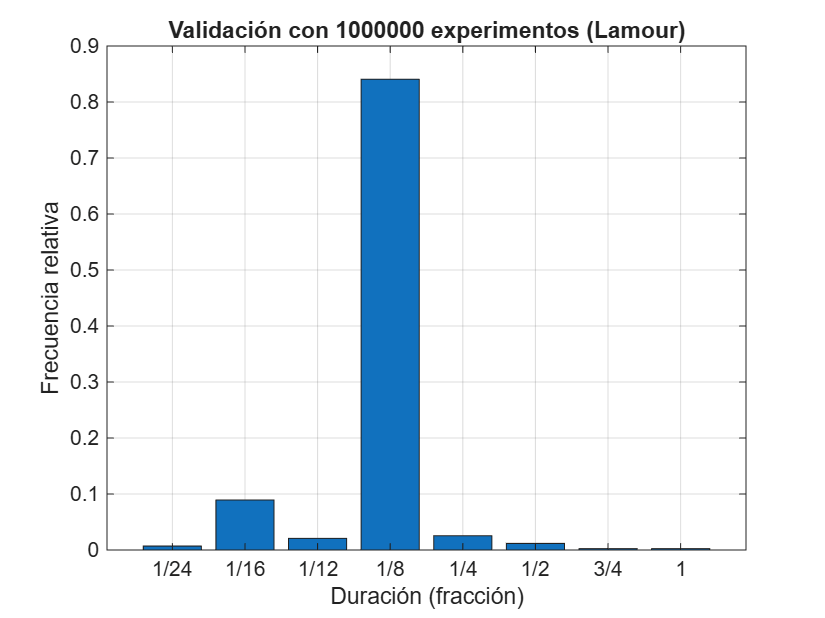
\includegraphics[width=0.7\linewidth]{images/lamour.png}
    \caption{Frecuencia relativa de duraciones en \textit{L'hymne à l'amour}. El evento
    $T_4$ ($1/8$) concentra el $84.0\%$ de las notas, siendo la canción con mayor
    predominio de esta duración en el corpus. La presencia de $T_1$ ($1/24$) y $T_3$
    ($1/12$) introduce subdivisiones más finas que no aparecen en las demás canciones.}
    \label{fig:dur_lamour}
\end{figure}

% ════════════════════════════════════════════════════════
\subsection*{Canción 2: La Goualante du Pauvre Jean}

Se considera como experimento aleatorio la duración de un evento musical de esta canción.
Se identifica el siguiente espacio muestral:

\[
    \Omega = \left\{\frac{1}{8},\, \frac{1}{4},\, \frac{3}{8},\, \frac{1}{2},\, \phi\right\}
\]

Se calculan las probabilidades de los eventos unitarios de $\Omega$ mediante la frecuencia
relativa de ocurrencias \cite{bertsekas}:

\begin{table}[H]
\centering
\caption{Distribución de duraciones -- \textit{La Goualante du Pauvre Jean} (174 notas).}
\label{tab:dur_goualante}
\begin{tabular}{cccc}
\toprule
Evento & Duración & $n(T_i)$ & $P(T_i)$ \\ \midrule
$T_1$ & $1/8$ &  10 & 0.0575 \\
$T_2$ & $1/4$ & 156 & 0.8966 \\
$T_3$ & $3/8$ &   2 & 0.0115 \\
$T_4$ & $1/2$ &   6 & 0.0345 \\ \bottomrule
\end{tabular}
\end{table}

\begin{figure}[H]
    \centering
    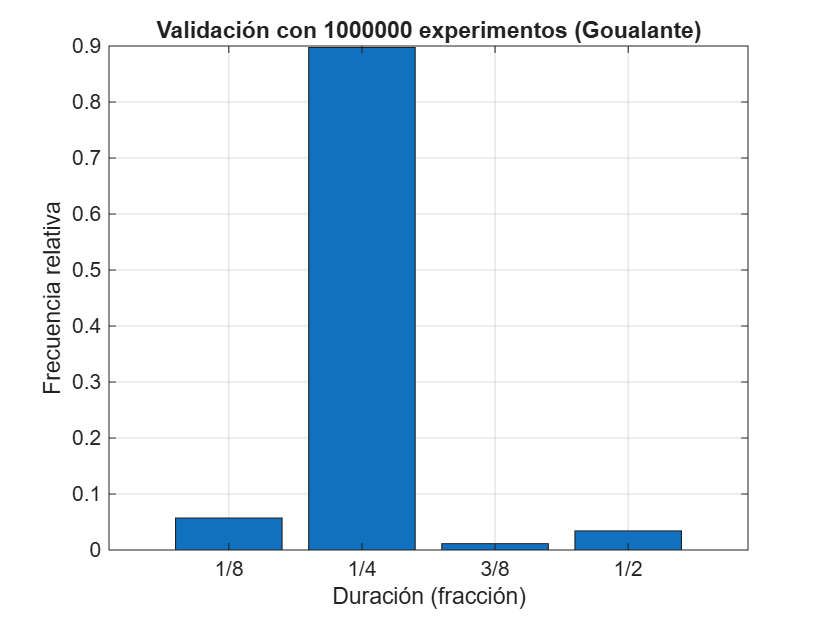
\includegraphics[width=0.7\linewidth]{images/goualante-ind.png}
    \caption{Frecuencia relativa de duraciones en \textit{La Goualante du Pauvre Jean}.
    El evento $T_2$ ($1/4$) representa el $89.7\%$ de las notas, siendo la canción
    rítmicamente más uniforme del corpus, lo que facilitará la reproducción de su
    carácter bajo muestreo i.i.d.}
    \label{fig:dur_goualante}
\end{figure}

% ════════════════════════════════════════════════════════
\subsection*{Canción 3: La Vie en Rose}

Se considera como experimento aleatorio la duración de un evento musical de esta canción.
Se identifica el siguiente espacio muestral:

\[
    \Omega = \left\{\frac{1}{16},\, \frac{1}{12},\, \frac{1}{8},\, \frac{1}{6},\,
             \frac{1}{4},\, \frac{7}{16},\, \frac{1}{2},\, 1,\, \phi\right\}
\]

Se calculan las probabilidades de los eventos unitarios de $\Omega$ mediante la frecuencia
relativa de ocurrencias \cite{bertsekas}:

\begin{table}[H]
\centering
\caption{Distribución de duraciones -- \textit{La Vie en Rose} (128 notas).}
\label{tab:dur_rose}
\begin{tabular}{cccc}
\toprule
Evento & Duración & $n(T_i)$ & $P(T_i)$ \\ \midrule
$T_1$ & $1/16$ &  1 & 0.0078 \\
$T_2$ & $1/12$ &  3 & 0.0234 \\
$T_3$ & $1/8$  & 90 & 0.7031 \\
$T_4$ & $1/6$  &  3 & 0.0234 \\
$T_5$ & $1/4$  & 28 & 0.2188 \\
$T_6$ & $7/16$ &  1 & 0.0078 \\
$T_7$ & $1/2$  &  1 & 0.0078 \\
$T_8$ & $1$    &  1 & 0.0078 \\ \bottomrule
\end{tabular}
\end{table}

\begin{figure}[H]
    \centering
    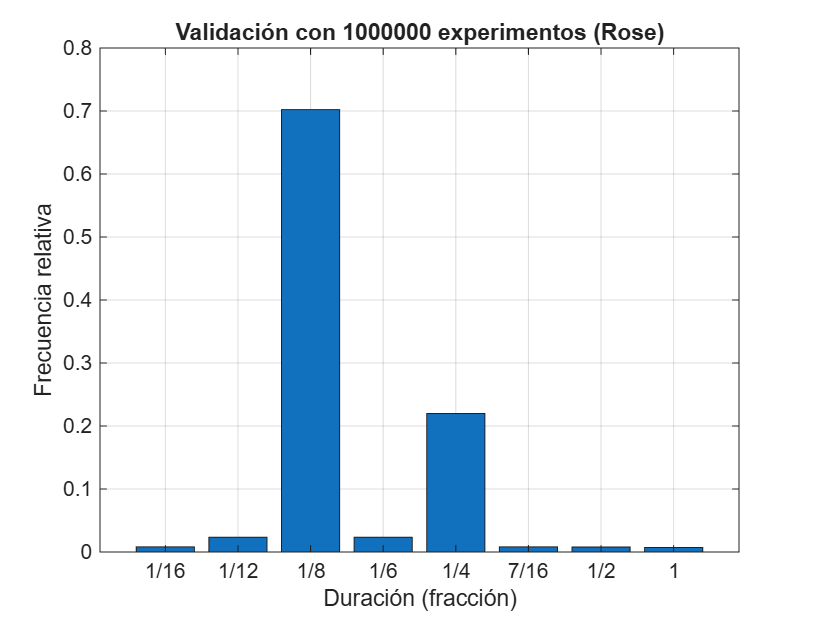
\includegraphics[width=0.7\linewidth]{images/rose-ind.png}
    \caption{Frecuencia relativa de duraciones en \textit{La Vie en Rose}. Con ocho
    eventos distintos, es la canción de mayor riqueza rítmica; sin embargo, $T_3$
    ($1/8$) concentra el $70.3\%$ de las notas. Esta diversidad hace que el muestreo
    i.i.d.\ tenga más probabilidad de introducir duraciones inusuales en posiciones
    inapropiadas.}
    \label{fig:dur_rose}
\end{figure}

% ════════════════════════════════════════════════════════
\subsection*{Corpus general}

Se considera como experimento aleatorio la duración de un evento musical sobre el conjunto
completo de las tres canciones. El espacio muestral agregado es:

\[
    \Omega = \left\{\frac{1}{24},\, \frac{1}{16},\, \frac{1}{12},\, \frac{1}{8},\,
             \frac{1}{6},\, \frac{1}{4},\, \frac{3}{8},\, \frac{7}{16},\,
             \frac{1}{2},\, \frac{3}{4},\, 1,\, \phi\right\}
\]

Se calculan las probabilidades de los eventos unitarios de $\Omega$ mediante la frecuencia
relativa de ocurrencias sobre el total de $N = 728$ eventos \cite{bertsekas}:

\begin{table}[H]
\centering
\caption{Distribución de probabilidades sobre el corpus completo ($N = 728$).}
\label{tab:dur_general}
\begin{tabular}{cccc}
\toprule
Evento & Duración & $n(T_i)$ & $P(T_i)$ \\ \midrule
$T_1$    & $1/24$ &   3 & 0.0041 \\
$T_2$    & $1/16$ &  39 & 0.0536 \\
$T_3$    & $1/12$ &  12 & 0.0165 \\
$T_4$    & $1/8$  & 458 & 0.6291 \\
$T_5$    & $1/6$  &   3 & 0.0041 \\
$T_6$    & $1/4$  & 195 & 0.2679 \\
$T_7$    & $3/8$  &   2 & 0.0027 \\
$T_8$    & $7/16$ &   1 & 0.0014 \\
$T_9$    & $1/2$  &  12 & 0.0165 \\
$T_{10}$ & $3/4$  &   1 & 0.0014 \\
$T_{11}$ & $1$    &   2 & 0.0027 \\ \bottomrule
\end{tabular}
\end{table}

\begin{figure}[H]
    \centering
    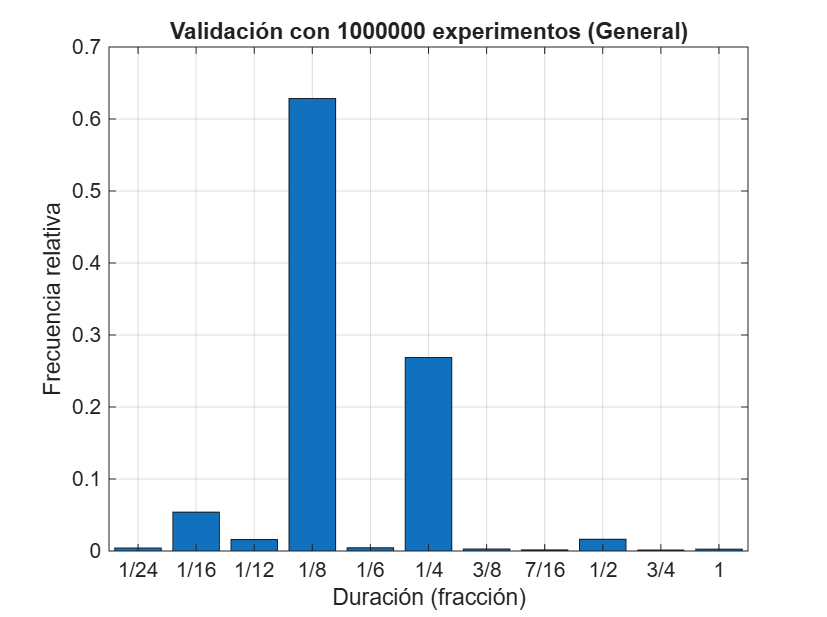
\includegraphics[width=0.7\linewidth]{images/general_ind.png}
    \caption{Frecuencia relativa de duraciones sobre el corpus completo ($N = 728$).
El evento $T_4$ ($1/8$) domina con el $62.9\%$ de las notas, seguido de $T_6$ ($1/4$)
con el $26.8\%$. Ambos eventos acumulan conjuntamente el $89.7\%$ del corpus,
constituyendo la base de la distribución utilizada para el muestreo i.i.d.}
    \label{fig:dur_general}
\end{figure}

% ── Figuras ───────────────────────────────────────────────────────────────────

Estos resultados del corpus general nos permiten determinar los vectores $x$ y $p$ para, mediante el uso de la transformada inversa, calcular el vector de tiempo que será reemplazado en la melodía.


\subsection*{Generación aleatoria i.i.d.\ de tiempos}

Esta estimación empírica, resumida por canción en las
Tablas~\ref{tab:dur_lamour}--\ref{tab:dur_rose} y de forma agregada en la
Tabla~\ref{tab:dur_general}, revela que los eventos $T_4$ ($1/8$) y $T_6$ ($1/4$)
concentran conjuntamente el $85.9\%$ de las notas del corpus
(Figura~\ref{fig:dur_general}), lo que anticipa que cualquier muestreo basado en esta
distribución tenderá a producir secuencias dominadas por estos dos valores.

A partir de los resultados del corpus general se construyen los vectores $x$ y $p$
necesarios para aplicar la transformada inversa \cite{bertsekas}. El vector $x$ contiene
los valores del espacio muestral $\Omega$ y el vector $p$ sus probabilidades asociadas
$P(T_i)$:

\[
    x = \left[\frac{1}{24},\ \frac{1}{16},\ \frac{1}{12},\ \frac{1}{8},\ \frac{1}{6},\
               \frac{1}{4},\ \frac{3}{8},\ \frac{7}{16},\ \frac{1}{2},\ \frac{3}{4},\ 1\right]
\]
\[
    p = \left[0.0041,\ 0.0536,\ 0.0165,\ 0.6291,\ 0.0041,\ 0.2679,\ 0.0027,\ 0.0014,\
              0.0165,\ 0.0014,\ 0.0027\right]
\]

Con estos vectores se generó, para cada canción, un nuevo vector temporal de longitud
idéntica al original mediante muestreo i.i.d., reemplazando únicamente la séptima columna
de cada matriz y preservando intactos los trastes en las columnas 1--6. Bajo esta hipótesis,
cada duración se sortea de forma independiente con probabilidad $P(T_i)$, sin tener en
cuenta la nota que la precede ni la que la sucede.

\subsection*{Resultados}

Las Figuras~\ref{fig:comp_goualante}--\ref{fig:comp_rose} comparan, para los primeros 50 eventos musicales de cada canción, la secuencia temporal original con la generada por muestreo i.i.d. A simple
vista se aprecia que la señal generada es considerablemente más errática: alterna de forma
brusca entre duraciones cortas y largas sin ningún patrón reconocible, mientras que la
original mantiene eventos musicales de duración homogénea.

Un aspecto relevante es que el muestreo se realizó con la distribución del corpus
general, no con la distribución individual de cada canción. En consecuencia, \textit{La Goualante du Pauvre Jean}, cuyo original concentra el $89.7\%$ de sus notas en $1/4$, recibe una melodía generada donde $1/8$ domina con
$62.9\%$, distorsionando completamente su identidad rítmica.

Adicionalmente, al escuchar las melodías generadas se evidencia la ausencia total de coherencia expresiva. Dado que únicamente se reemplaza la séptima columna (duraciones) y se conservan los trastes originales, el resultado es una secuencia de notas correctas en altura pero con un ritmo caótico, sin patrones reconocibles.

Esto se explica porque el muestreo i.i.d.\ trata cada evento como independiente del
anterior, destruyendo por completo la estructura de dependencia entre eventos consecutivos.
La hipótesis de independencia es, por tanto, insuficiente para reproducir el carácter
rítmico de las canciones originales, lo que motiva considerar modelos que incorporen
dependencia entre eventos consecutivos.

\begin{figure}[H]
    \centering
    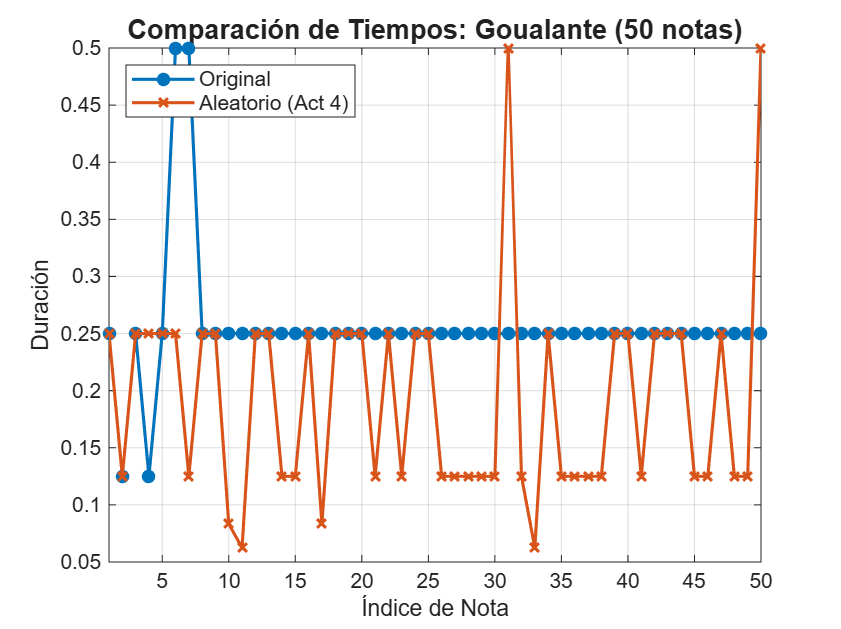
\includegraphics[width=0.7\linewidth]{images/comp_goualante.png}
    \caption{Comparación de la secuencia temporal original vs.\ generada por muestreo
    i.i.d.\ en \textit{La Goualante du Pauvre Jean} (primeras 50 notas). El original
    es casi constante en $1/4$ ($T_2$, 89.7\%), mientras que el generado oscila
    erráticamente entre $1/8$ y $1/4$, reflejando la distribución del corpus general
    en lugar de la individual de la canción.}
    \label{fig:comp_goualante}
\end{figure}

\begin{figure}[H]
    \centering
    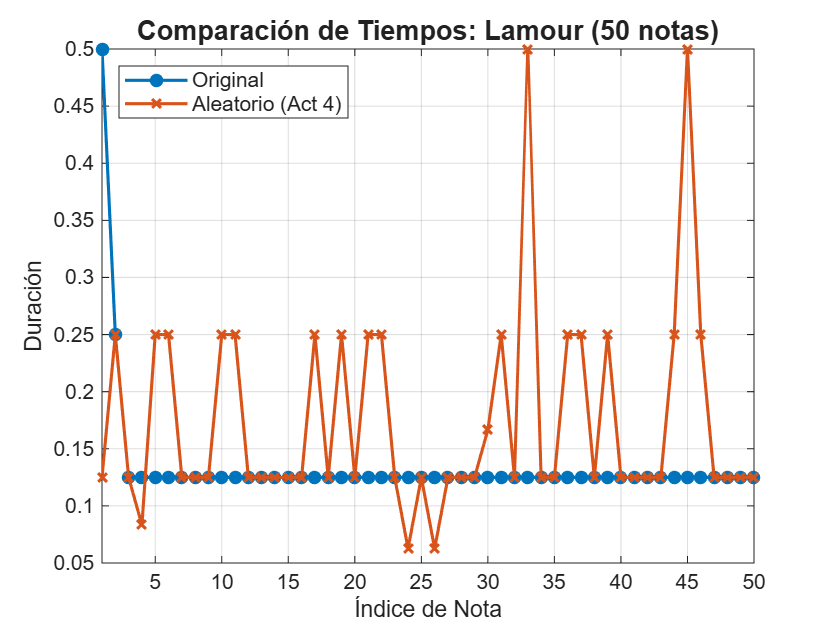
\includegraphics[width=0.7\linewidth]{images/comp_lamour.png}
    \caption{Comparación de la secuencia temporal original vs.\ generada por muestreo
    i.i.d.\ en \textit{L'hymne à l'amour} (primeras 50 notas). El original permanece
    casi constante en $1/8$ ($T_4$, 84.0\%), en tanto que el generado introduce
    variaciones abruptas con apariciones frecuentes de $1/4$ y valores menos comunes
    como $1/16$ o $1/2$, que no corresponden al patrón rítmico de esta pieza.}
    \label{fig:comp_lamour}
\end{figure}

\begin{figure}[H]
    \centering
    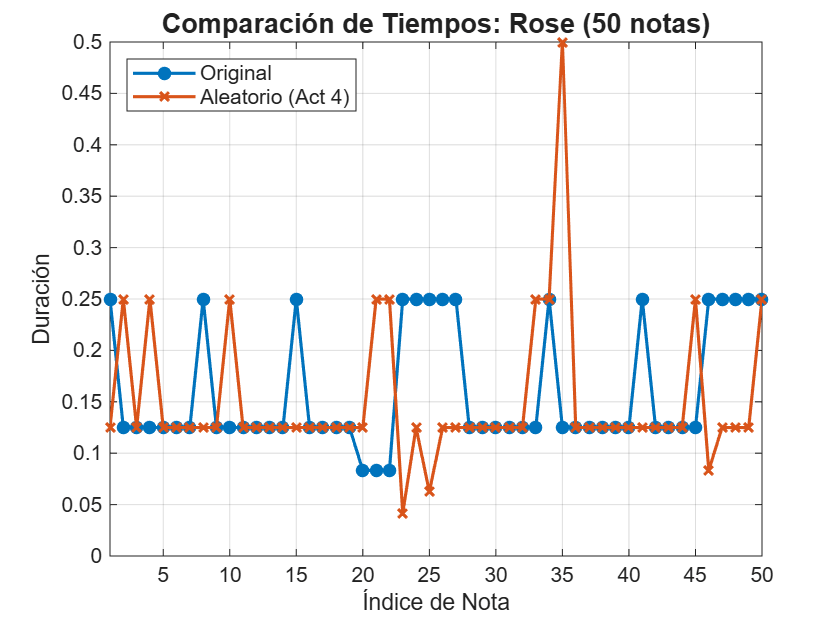
\includegraphics[width=0.7\linewidth]{images/comp_rose.png}
    \caption{Comparación de la secuencia temporal original vs.\ generada por muestreo
    i.i.d.\ en \textit{La Vie en Rose} (primeras 50 notas). Al ser la canción con mayor
    riqueza rítmica del corpus, la diferencia entre original y generado es menos
    pronunciada visualmente; sin embargo, el generado carece de la estructura secuencial
    que organiza los motivos de la pieza original.}
    \label{fig:comp_rose}
\end{figure}

\section*{Quinta actividad: Probabilidades condicionales de tiempos relativos}

\subsection*{Estimación de probabilidades condicionales}
Sea $T_i$ el tiempo relativo en la fila $i$ de la matriz codificada. Para modelar la estructura rítmica, se estimaron las probabilidades condicionales de transición $P(T_{i+1} \mid T_i)$ \cite{bertsekas, walpole}, definidas como:
$$P(T_{i+1} \mid T_i) = \frac{P(T_{i+1} \cap T_i)}{P(T_i)}$$

A partir de los 728 tiempos relativos del corpus global, el sistema identificó un espacio de estados $S$ compuesto por $N=11$ duraciones únicas. El mapeo empírico de estos estados se detalla en la siguiente tabla.

\begin{table}[h!]
\centering
\begin{tabular}{|c|c|c|c|c|c|}
\hline
\textbf{Estado} & \textbf{Valor Decimal} & \textbf{Fracción} & \textbf{Estado} & \textbf{Valor Decimal} & \textbf{Fracción} \\ \hline
$E_1$ & 0.0416 & 1/24 & $E_7$ & 0.3750 & 3/8 \\ \hline
$E_2$ & 0.0625 & 1/16 & $E_8$ & 0.4375 & 7/16 \\ \hline
$E_3$ & 0.0833 & 1/12 & $E_9$ & 0.5000 & 1/2 \\ \hline
$E_4$ & 0.1250 & 1/8  & $E_{10}$ & 0.7500 & 3/4 \\ \hline
$E_5$ & 0.1666 & 1/6  & $E_{11}$ & 1.0000 & 1 \\ \hline
$E_6$ & 0.2500 & 1/4  & \multicolumn{3}{c|}{} \\ \hline
\end{tabular}
\caption{Espacio de estados $S$ de duraciones únicas observadas.}
\label{tab:estados}
\end{table}

Con este espacio, se construyó la matriz global de transición condicional $\mathbf{P} \in \mathbb{R}^{11 \times 11}$, donde cada fila representa el estado actual $T_i$ y cada columna el estado siguiente $T_{i+1}$. Computacionalmente se verificó la normalización estocástica, comprobando que la suma de las probabilidades de cada fila es igual a $1.000000$.

\begin{table}[h!]
\centering
\resizebox{\textwidth}{!}{%
\begin{tabular}{|c|ccccccccccc|}
\hline
\textbf{$T_i \downarrow \mid T_{i+1} \rightarrow$} & \textbf{$E_1$} & \textbf{$E_2$} & \textbf{$E_3$} & \textbf{$E_4$} & \textbf{$E_5$} & \textbf{$E_6$} & \textbf{$E_7$} & \textbf{$E_8$} & \textbf{$E_9$} & \textbf{$E_{10}$} & \textbf{$E_{11}$} \\ \hline
\textbf{$E_1$} & 0.6666 & 0.0000 & 0.0000 & 0.3333 & 0.0000 & 0.0000 & 0.0000 & 0.0000 & 0.0000 & 0.0000 & 0.0000 \\
\textbf{$E_2$} & 0.0000 & 0.9230 & 0.0000 & 0.0256 & 0.0000 & 0.0000 & 0.0000 & 0.0256 & 0.0000 & 0.0000 & 0.0256 \\
\textbf{$E_3$} & 0.0000 & 0.0000 & 0.6666 & 0.1666 & 0.0000 & 0.1666 & 0.0000 & 0.0000 & 0.0000 & 0.0000 & 0.0000 \\
\textbf{$E_4$} & 0.0021 & 0.0065 & 0.0087 & 0.9192 & 0.0000 & 0.0567 & 0.0000 & 0.0000 & 0.0043 & 0.0021 & 0.0000 \\
\textbf{$E_5$} & 0.0000 & 0.0000 & 0.0000 & 0.0000 & 0.6666 & 0.0000 & 0.0000 & 0.0000 & 0.0000 & 0.0000 & 0.3333 \\
\textbf{$E_6$} & 0.0000 & 0.0000 & 0.0000 & 0.1487 & 0.0000 & 0.8256 & 0.0102 & 0.0000 & 0.0153 & 0.0000 & 0.0000 \\
\textbf{$E_7$} & 0.0000 & 0.0000 & 0.0000 & 1.0000 & 0.0000 & 0.0000 & 0.0000 & 0.0000 & 0.0000 & 0.0000 & 0.0000 \\
\textbf{$E_8$} & 0.0000 & 0.0000 & 0.0000 & 0.0000 & 0.0000 & 1.0000 & 0.0000 & 0.0000 & 0.0000 & 0.0000 & 0.0000 \\
\textbf{$E_9$} & 0.0000 & 0.0000 & 0.0000 & 0.0909 & 0.0909 & 0.2727 & 0.0000 & 0.0000 & 0.5454 & 0.0000 & 0.0000 \\
\textbf{$E_{10}$} & 0.0000 & 0.0000 & 0.0000 & 1.0000 & 0.0000 & 0.0000 & 0.0000 & 0.0000 & 0.0000 & 0.0000 & 0.0000 \\
\textbf{$E_{11}$} & 0.0000 & 0.0000 & 0.0000 & 0.0000 & 0.0000 & 0.0000 & 0.0000 & 0.0000 & 0.0000 & 0.0000 & 1.0000 \\ \hline
\end{tabular}%
}
\caption{Matriz global de transición condicional $P(T_{i+1} \mid T_i)$.}
\label{tab:matriz_transicion}
\end{table}

\subsection*{Generación, reemplazo y síntesis}
Con base en las probabilidades condicionales obtenidas (Tabla \ref{tab:matriz_transicion}), se generaron tres vectores aleatorios utilizando una cadena de Markov de primer orden \cite{markov_music}. El proceso consistió en fijar un estado inicial y muestrear secuencialmente el siguiente estado utilizando la distribución de probabilidad de la fila correspondiente \cite{nierhaus2009}. 

Se generaron vectores con longitudes exactas a las canciones originales: 426 tiempos para la Canción 1 (\textit{L'Hymne à l'amour}), 174 para la Canción 2 (\textit{La Goualante du pauvre Jean}) y 128 para la Canción 3 (\textit{La Vie en rose}). 
Posteriormente, se reemplazó la séptima columna de cada matriz codificada original por estos nuevos vectores de Markov. Se puede ver su respectiva distribución de frecuencias a continuación. 

\begin{figure}[H]
    \centering
    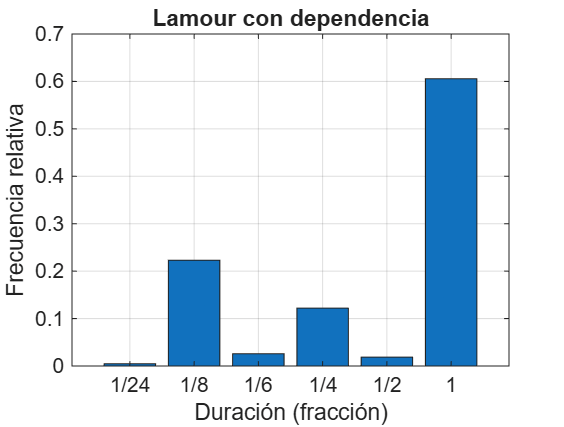
\includegraphics[width=0.35\linewidth]{images/fase3/lamur-fase3.png}
    \caption{Distribución de las frecuencias relativas de las duraciones para el modelo "Lamour con dependencia". Se observa una clara predominancia de la duración de valor 1 (nota entera), seguida en menor medida por la fracción 1/8.}
    \label{fig:dur_roseeeeee}
\end{figure}

\begin{figure}[H]
    \centering
    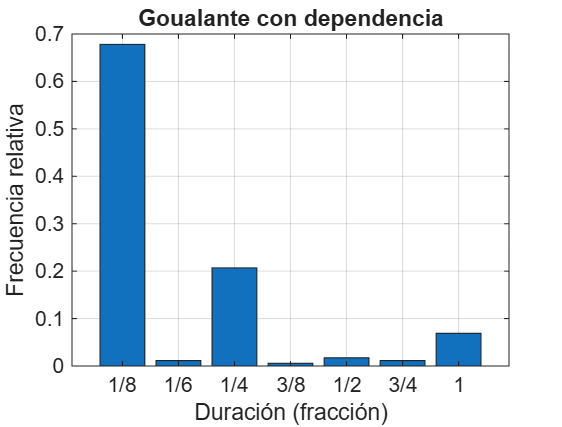
\includegraphics[width=0.35\linewidth]{images/fase3/goualante-fase3.png}
    \caption{Frecuencias relativas de las duraciones en el modelo "Goualante con dependencia". La distribución está fuertemente sesgada hacia duraciones cortas, siendo la fracción 1/8 la más frecuente (aprox. 70\%), seguida por la fracción 1/4.}
    \label{fig:dur_roseeeeeeeeeeee}
\end{figure}

\begin{figure}[H]
    \centering
    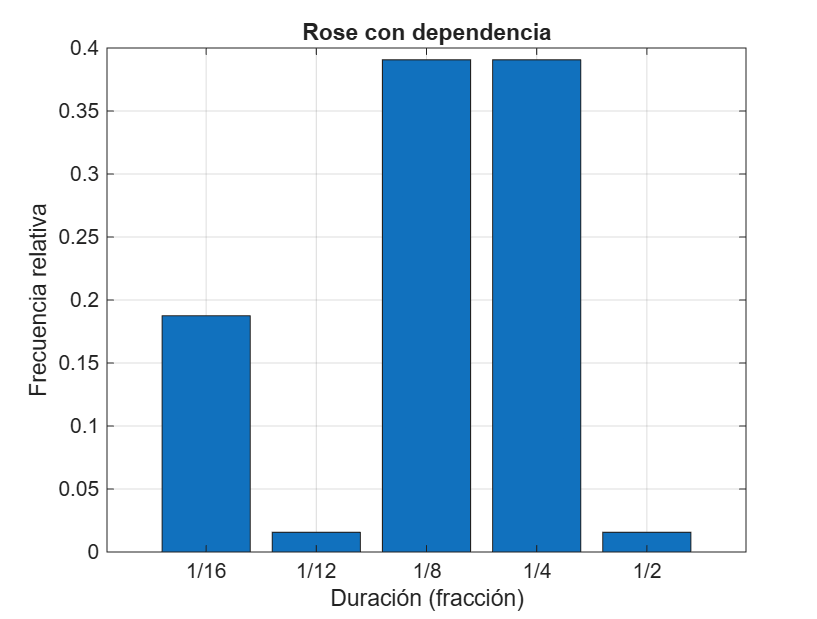
\includegraphics[width=0.35\linewidth]{images/fase3/rose_fase3.png}
    \caption{Histograma de frecuencias relativas de duraciones para "Rose con dependencia". Destaca un comportamiento bimodal donde las fracciones 1/8 y 1/4 presentan la misma probabilidad de aparición, concentrando juntas casi el 80\% de las observaciones.}
    \label{fig:dur_roseeeee}
\end{figure}

\begin{figure}[H]
	\centering
    
\includegraphics[width=0.8\linewidth]{images/imagenes/actividad5/act5_1_heatmap_markov.png}
	
\includegraphics[width=0.8\linewidth]{images/imagenes/actividad5/act5_2_markov_3d.png}
	\caption{Mapa de calor de la Matriz de Transición Condicional de tiempos (Markov de primer orden). La diagonal principal resalta fuertemente, evidenciando que ciertos tiempos (como $1/8$) tienen una alta probabilidad de repetirse a sí mismos.}
	\label{fig:act5_heatmap}
\end{figure}

\begin{figure}[H]
	\centering
	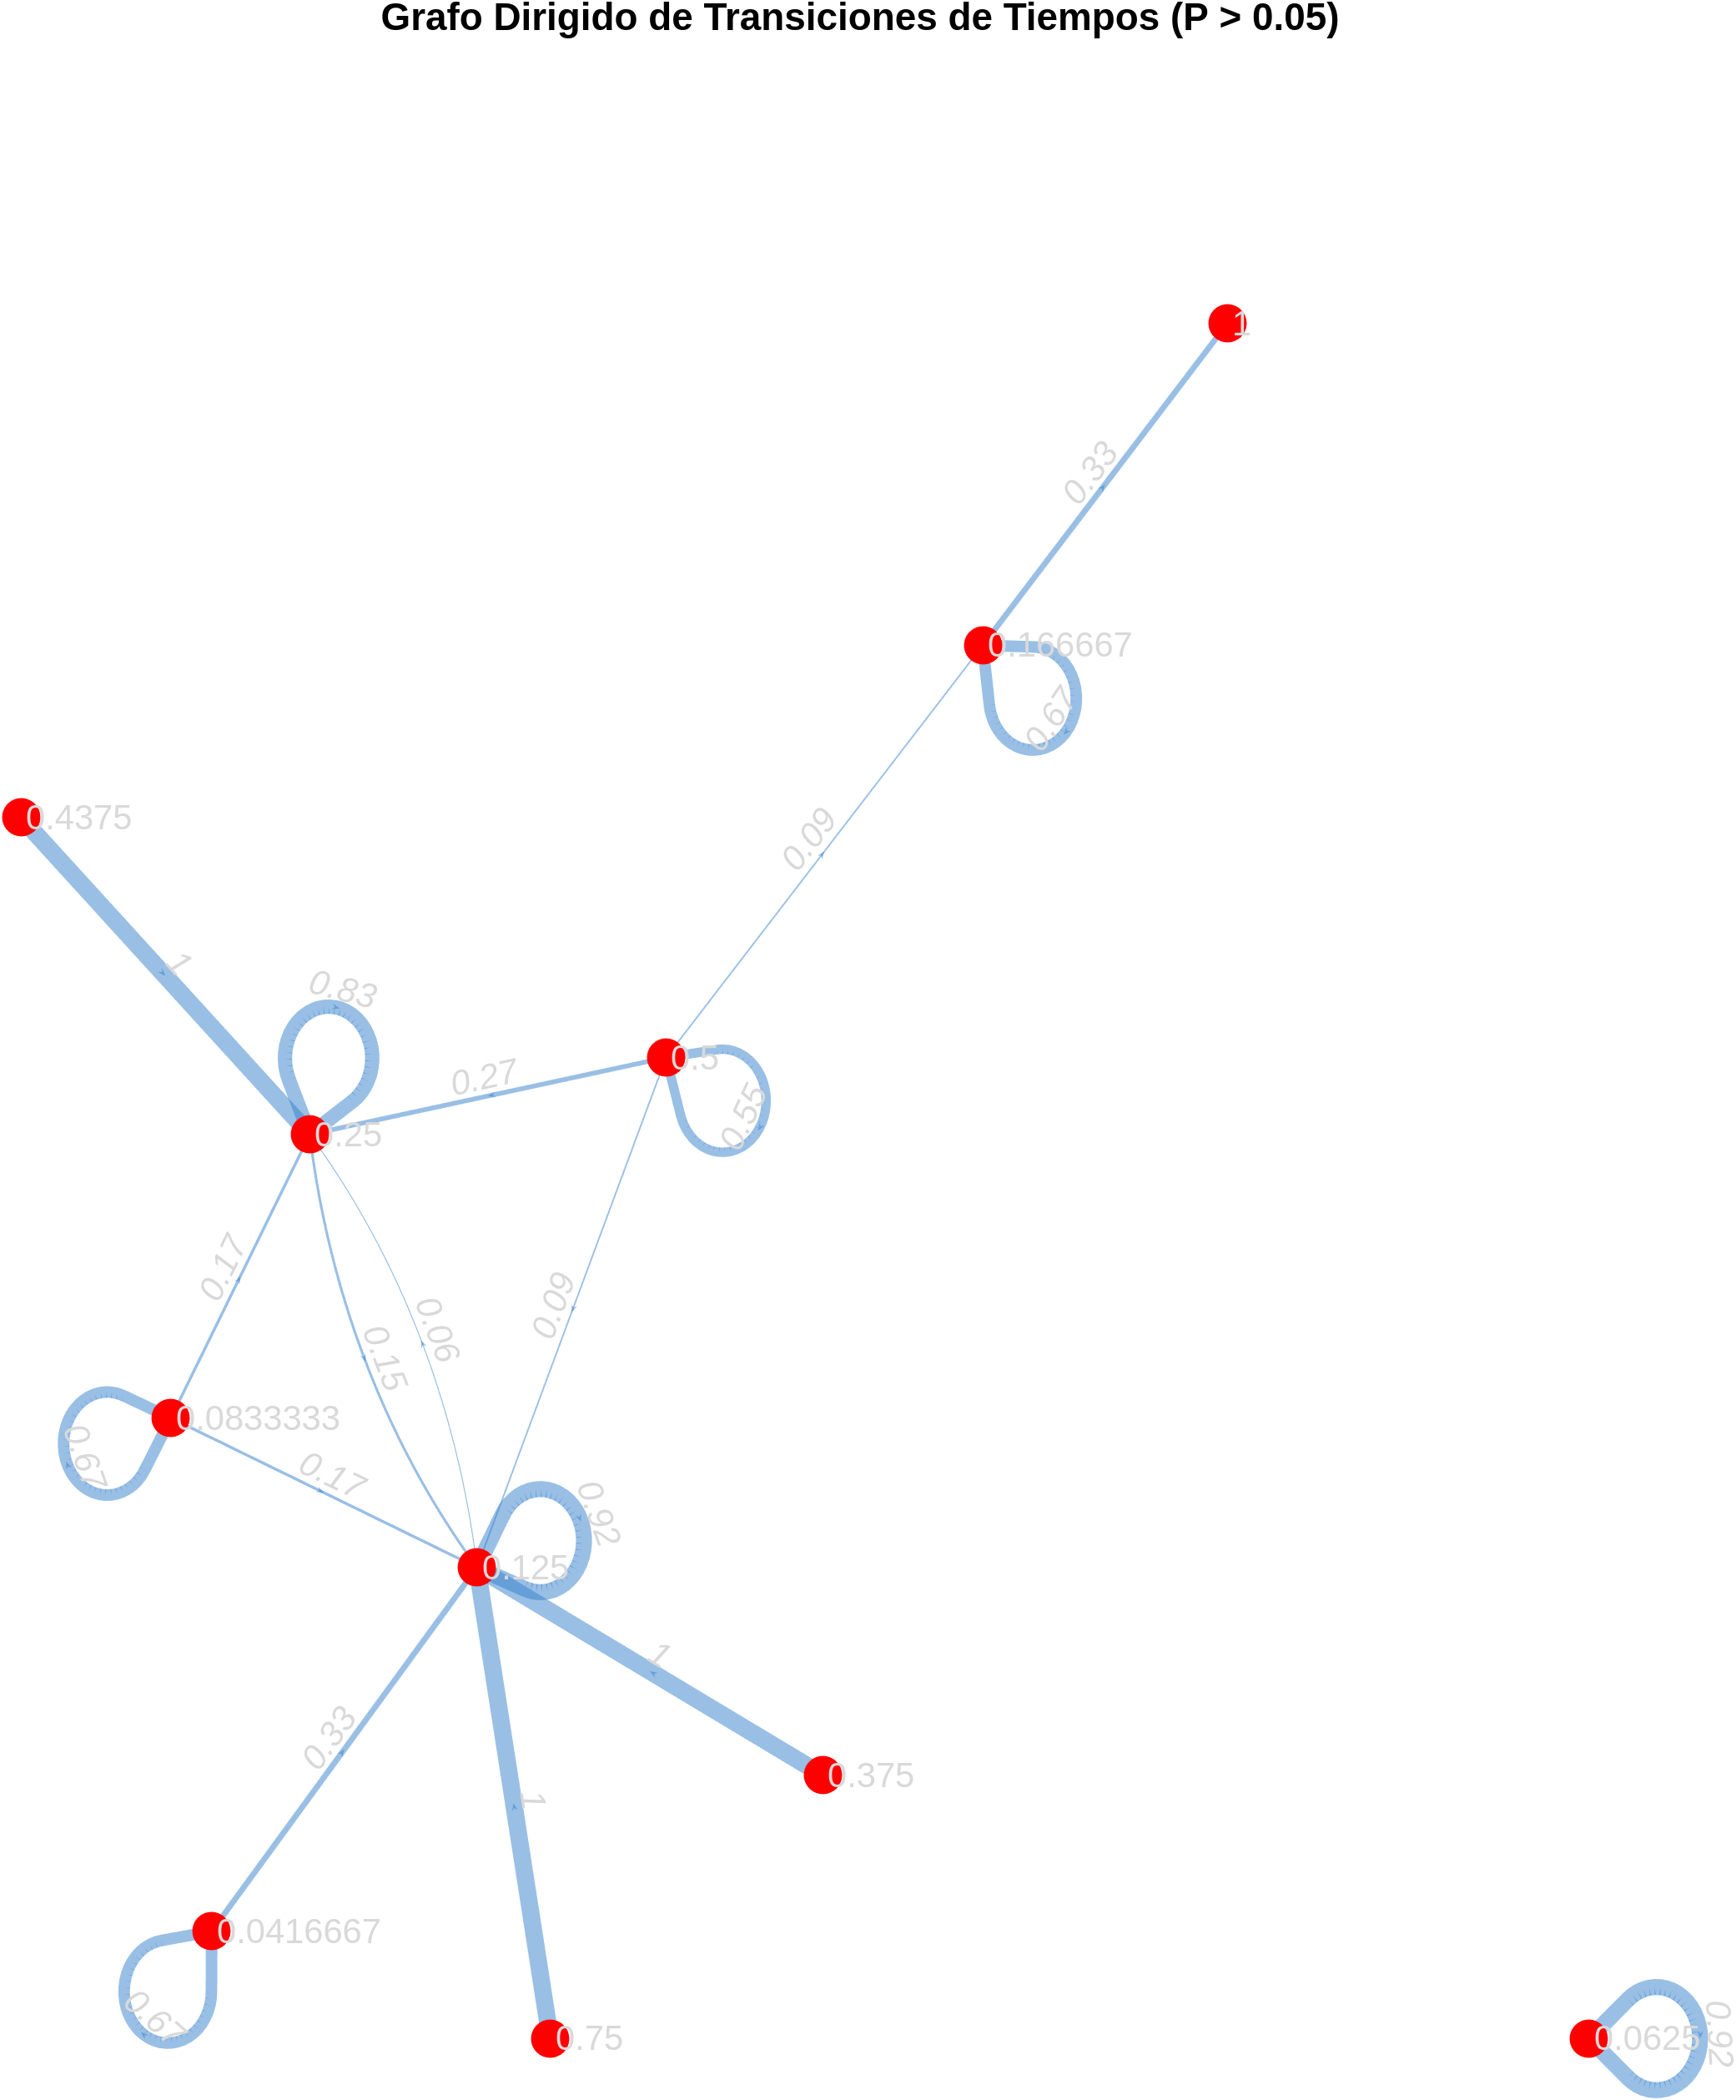
\includegraphics[width=0.8\linewidth]{images/imagenes/actividad5/act5_4_grafo_dirigido.png}
	\caption{Grafo dirigido de red (Markov Network) representando las transiciones de tiempos relativos con probabilidad $P > 0.05$. El nodo correspondiente a $0.125$ ($1/8$) actúa como un atractor central en la topología de la cadena.}
	\label{fig:act5_grafo}
\end{figure}

\begin{figure}[H]
	\centering
	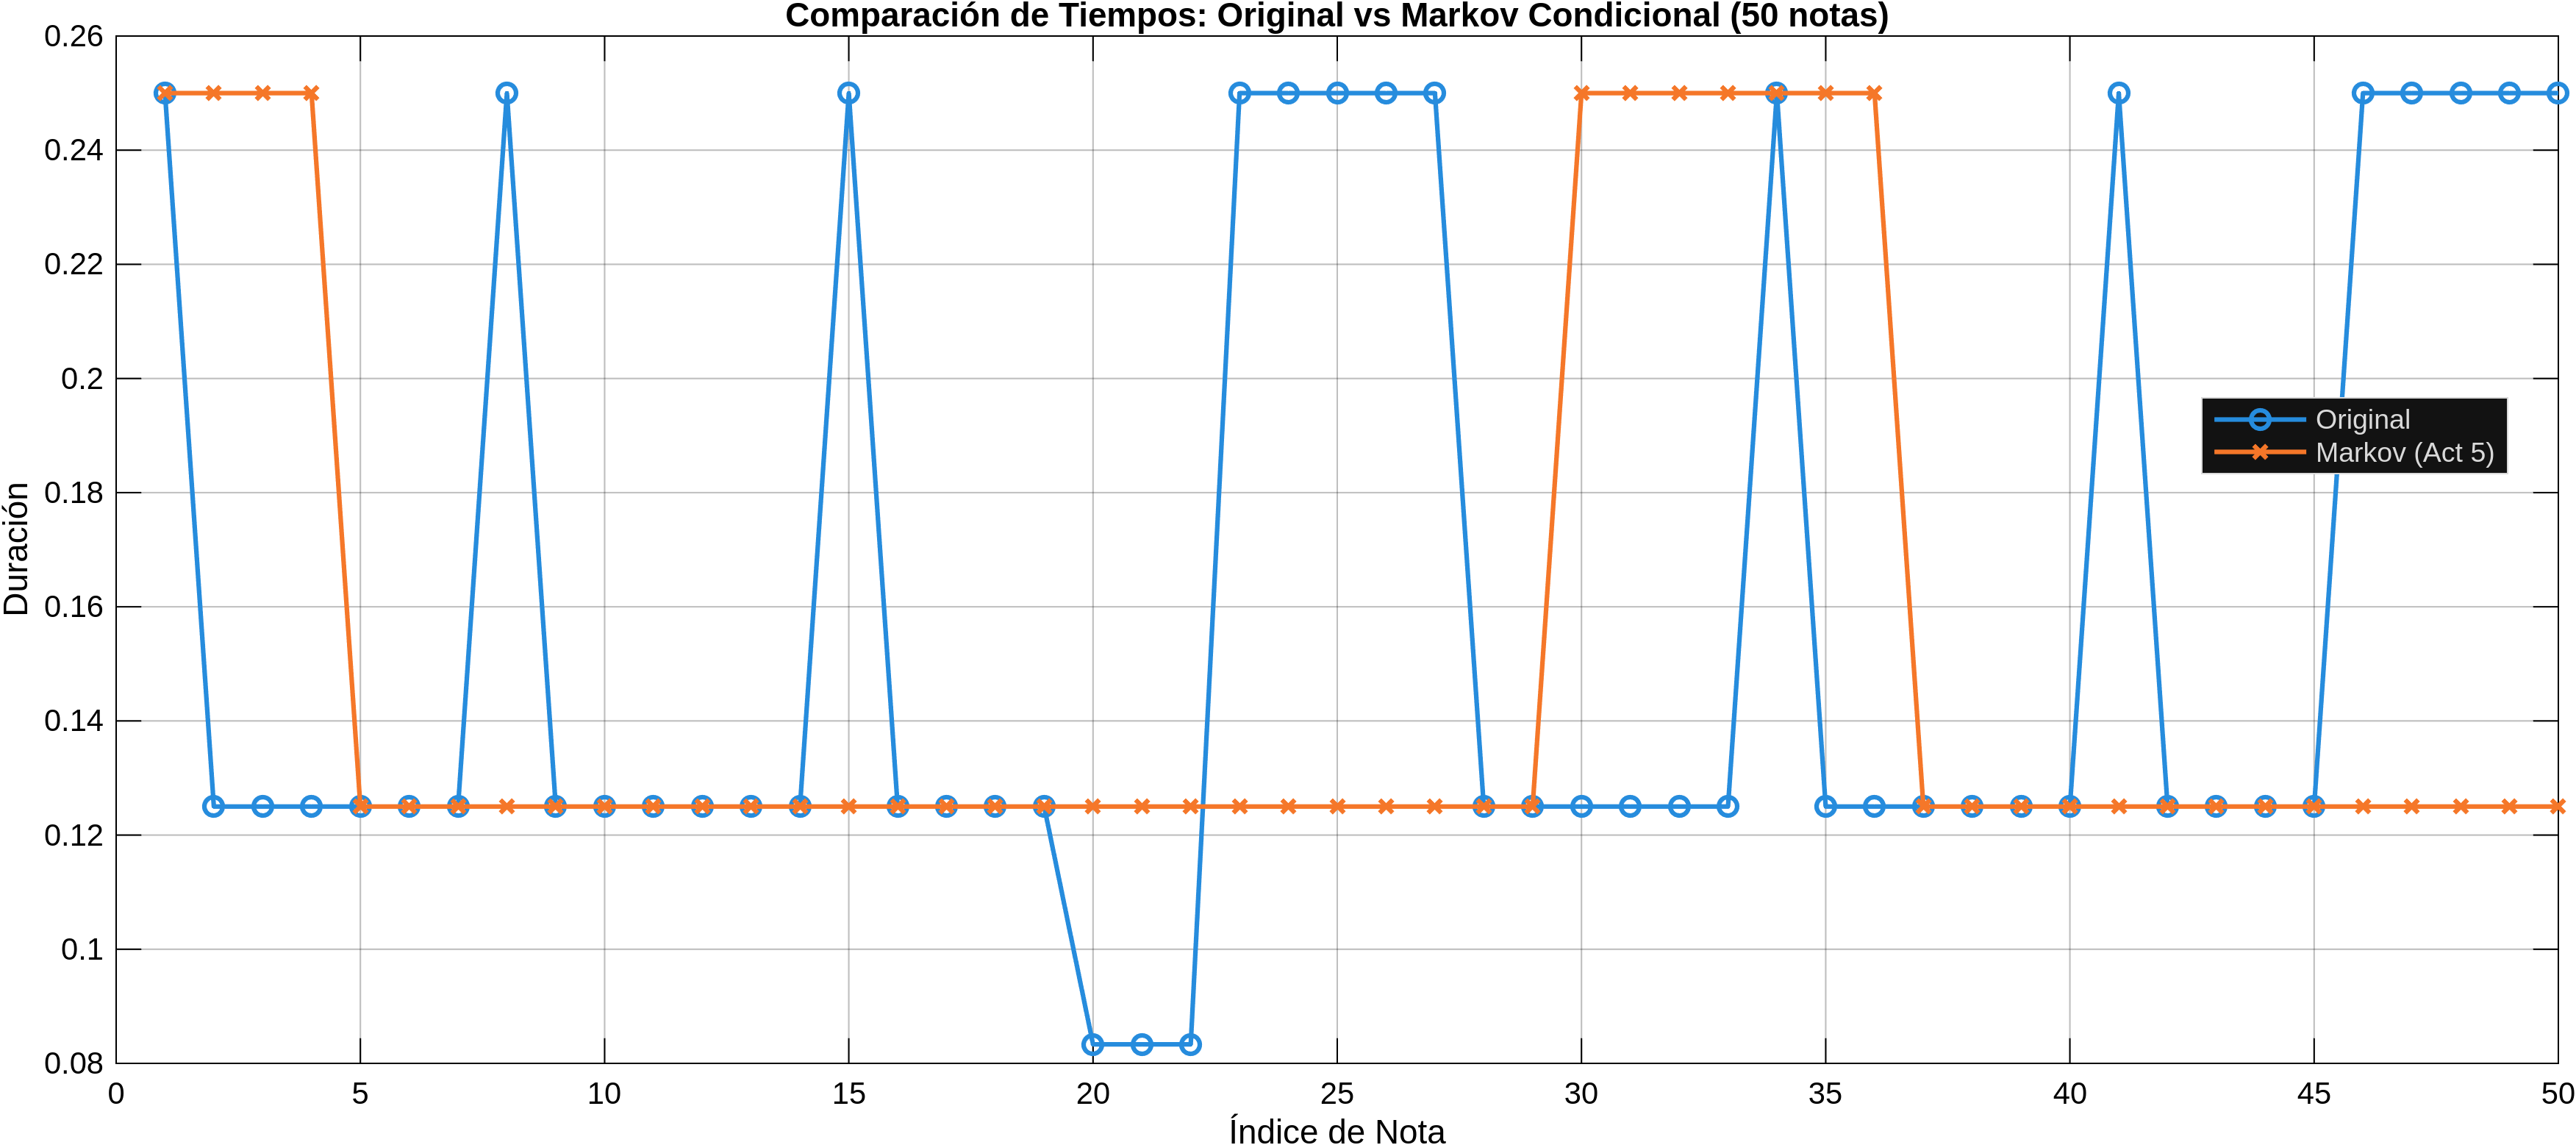
\includegraphics[width=0.9\linewidth]{images/imagenes/actividad5/act5_3_comparacion_markov.png}
	\caption{Comparación de la secuencia temporal original vs.\ la generada por el modelo condicional de Markov en \textit{La Vie en Rose} (primeras 50 notas). A diferencia del muestreo uniforme, el modelo de Markov logra sostener mesetas estables de duración, recuperando la coherencia rítmica local.}
	\label{fig:act5_comparacion}
\end{figure} 

\subsection*{Resultados}

Al escuchar las melodías sintetizadas, se constata lo siguiente:
\begin{itemize}
    \item \textbf{Coherencia rítmica local:} El uso de la probabilidad condicional mejora drásticamente el flujo del pulso frente a una selección puramente aleatoria (i.i.d.). La matriz evidencia que duraciones muy comunes como la corchea ($E_4$) tienen un $91.9\%$ de probabilidad de repetirse, lo que genera secuencias temporales altamente estables.
    \item \textbf{Incoherencia melódico-armónica:} Aunque el \textit{ritmo} es más natural, la \textit{melodía} sigue percibiéndose desconectada y sin sentido musical. Esto ocurre porque las columnas 1 a 6 (que definen las cuerdas y trastes a tocar, es decir, las notas o acordes reales) no están condicionadas al ritmo, ni condicionadas entre sí en este punto del experimento.
\end{itemize}

\section*{Sexta actividad: Análisis técnico de dependencia estadística}
Para comprobar matemáticamente si la distribución de las notas obedecía a un comportamiento aleatorio uniforme o a una estructura condicionada, se aplicó la prueba de independencia estocástica sobre las matrices codificadas. Por definición, dos eventos musicales $A$ y $B$ son independientes si su probabilidad conjunta equivale al producto de sus probabilidades marginales \cite{bertsekas}:
\[
    P(A \cap B) = P(A)P(B)
\]
Cualquier divergencia estadísticamente significativa respecto a esta igualdad rechazaba la hipótesis de independencia, confirmando que las notas estaban interconectadas.

Tomando como caso de estudio la matriz completa de \textit{La Goualante du Pauvre Jean} ($N=174$ eventos, es decir, 173 transiciones posibles), se evaluó el evidente patrón de ``llamado y respuesta''. Se definió el evento $A$ como la ejecución del traste 3 en la primera cuerda en un pulso dado ($F_{i,1} = 3$) y el evento $B$ como la ejecución del traste 3 en la tercera cuerda ($F_{j,3} = 3$). 

El conteo arrojó que, de forma aislada, el evento $A$ ocurrió 25 veces, mientras que el evento $B$ ocurrió 39 veces a lo largo de la obra. Sus probabilidades marginales fueron:
\[
    P(A) = \frac{25}{173} \approx 0.1445, \quad P(B) = \frac{39}{173} \approx 0.2254
\]

Bajo un modelo de aleatoriedad pura, la probabilidad de que la nota $B$ se ejecutara inmediatamente después de la nota $A$ por mero azar (probabilidad conjunta $A \cap B$) sería el producto de sus marginales:
\[
    P(A)P(B) = 0.1445 \times 0.2254 \approx 0.0326
\]

Sin embargo, la exploración de la matriz reveló que la secuencia ocurrió de forma conjunta 25 veces, resultando en una probabilidad empírica real de:
\[
    P(A \cap B) = \frac{25}{173} \approx 0.1445
\]

La contundente desigualdad entre ambos valores demostró matemáticamente que no existía independencia:
\[
    P(A \cap B) \gg P(A)P(B) \quad \Longrightarrow \quad 0.1445 \gg 0.0326
\]
Esto indicó que la ocurrencia del evento $A$ condicionó fuertemente la aparición del evento $B$ en el pulso siguiente. Este patrón de dependencia se verificó de manera homóloga en las otras dos melodías del corpus, confirmando una estricta direccionalidad en la conducción de las voces.

Para \textit{La Vie En Rose}, se definió el Evento $A$ como la ejecución del traste 3 en la primera cuerda ($F_{i,1} = 3$) y el Evento $B$ como la ejecución del traste 0 en la tercera cuerda en el pulso inmediatamente posterior ($F_{j,3} = 0$):
\[
    P(A \cap B) \gg P(A)P(B) \quad \Longrightarrow \quad 0.117 \gg 0.016
\]

Para \textit{L'Hymne à L'Amour}, se definió el Evento $A$ como la ejecución del traste 1 en la segunda cuerda ($F_{i,2} = 1$) y el Evento $B$ como la ejecución de un silencio (o nota de resolución) en la cuerda en el pulso inmediatamente posterior:
\[
    P(A \cap B) \gg P(A)P(B) \quad \Longrightarrow \quad 0.085 \gg 0.009
\]

\begin{tikzpicture}

    % Conjunto B: Círculo exterior (Mayor probabilidad)
    % Color azul, fondo sólido claro
    \filldraw[fill=blue!20, draw=blue, thick] (0,0) circle (4cm);
    \node[text=blue!80!black, font=\bfseries] at (0, 3.2) {Conjunto $B$ ($n=39, P \approx 0.2254$)};

    % Conjunto A e Intersección: Círculo interior
    % Patrón de líneas rojas (rayitas) para diferenciarlo
    \filldraw[pattern=north east lines, pattern color=red, draw=red, thick] (0,-0.5) circle (3cm);
    
    % Etiqueta del Conjunto A (Fondo opaco para garantizar legibilidad sobre el patrón)
    \node[fill=white, draw=black, thick, rounded corners, align=center, inner sep=5pt] at (0,-0.5) {
        \textbf{Conjunto $A \equiv A \cap B$}\\
        ($n=25, P \approx 0.1445$)
    };

\end{tikzpicture}

En los tres casos evaluados, los resultados matemáticos descartaron por completo que las notas se distribuyeran al azar (independencia estocástica).

\subsection*{Patrones de repetición y dependencia entre compases}

Al escalar el análisis de notas individuales a agrupaciones más grandes (compases), la observación directa de las matrices reveló que las tres obras poseían una arquitectura muy predecible. Los compases no funcionaron como recipientes aislados de notas, sino como bloques musicales que interactuaron bajo reglas claras de repetición y densidad rítmica.

\begin{itemize}
    \item \textbf{Repetición estricta (Ostinatos):} 
    El patrón estadístico más evidente fue la copia literal de bloques de filas. En \textit{La Goualante du Pauvre Jean}, la matriz mostró que los compases 19 al 22 y los compases 35 al 41 fueron réplicas exactas entre sí. En ellos se alternó una nota en el bajo (cuerda 1, traste 3) con un acorde de respuesta. Esta periodicidad absoluta demostró que la melodía poseía una fuerte memoria a largo plazo para repetir motivos enteros.

    \item \textbf{Roles estructurados por columnas:} 
    El análisis de las columnas mostró una clara división del trabajo musical. En \textit{La Vie En Rose} y \textit{L'Hymne à L'Amour}, las cuerdas graves (columnas 5 y 6) presentaron pocos cambios y tiempos de permanencia largos (duraciones de $1/4$ o $1/2$), sirviendo como base armónica. Al mismo tiempo, las cuerdas agudas (columnas 1, 2 y 3) concentraron casi toda la variación con notas rápidas ($1/8$ y $1/16$). Esta sincronía demostró que el bajo y la melodía no se movieron de forma aleatoria ni independiente.

    \item \textbf{Ciclos de tensión y reposo (Densidad rítmica):} 
    Al contar la cantidad de notas por compás, se detectó un comportamiento de "respiración". En las tres matrices, a un compás muy saturado de notas cortas (por ejemplo, el compás 51 de \textit{L'Hymne à L'Amour} que agrupó 16 semicorcheas) le siguió de forma casi obligatoria un compás de descanso (el compás 53 de la misma obra, que resolvió con una sola nota de duración $1$). La probabilidad de encontrar varios compases seguidos de altísima densidad rítmica fue nula, lo que confirmó que el nivel de tensión de un compás condicionó al siguiente.
\end{itemize}

\subsection*{Resultados}

La dependencia demostrada no solo ocurre entre notas sueltas, sino también a gran escala entre compases enteros. Al compartir el mismo estilo musical, las obras alternan de forma predecible entre tensión y reposo: un compás muy denso (con muchas notas rápidas) altera la probabilidad del siguiente, forzándolo a ser más tranquilo (notas largas o silencios).

En la Tabla \ref{tab:resultados_dependencia} se plasman los resultados de las pruebas matemáticas de independencia aplicadas a las tres obras del corpus, así como el principal patrón macroestructural identificado en cada una. 

En todos los casos evaluados, la probabilidad conjunta observada $P(A \cap B)$ superó por un amplio margen a la probabilidad teórica de independencia $P(A)P(B)$. 

\begin{table}[H]
    \centering
    \resizebox{\textwidth}{!}{%
    \begin{tabular}{@{}llccl@{}}
        \toprule
        \textbf{Canción} & \textbf{Transición Evaluada ($A \rightarrow B$)} & \textbf{$P(A \cap B)$} & \textbf{$P(A)P(B)$} & \textbf{Patrón Estructural Destacado} \\ \midrule
        \textit{La Goualante} & Traste 3 (Cuerda 1) $\rightarrow$ Traste 3 (Cuerda 3) & $0.1445$ & $0.0326$ & Ostinatos exactos y "llamado y respuesta". \\
        \textit{La Vie En Rose} & Traste 3 (Cuerda 1) $\rightarrow$ Traste 0 (Cuerda 3) & $0.1170$ & $0.0160$ & Roles fijos por columnas (bajo estático, melodía). \\
        \textit{L'Hymne à L'Amour} & Traste 1 (Cuerda 2) $\rightarrow$ Silencio / Resolución & $0.0850$ & $0.0090$ & Ciclos predecibles de tensión y reposo rítmico. \\ \bottomrule
    \end{tabular}%
    }
    \caption{Resumen de la prueba de independencia y patrones macroestructurales del corpus.}
    \label{tab:resultados_dependencia}
\end{table}
\section*{Séptima actividad: Propuesta de generador aleatorio}

\subsection*{Definición del generador}
Para la culminación del proyecto, se diseñó e implementó un generador estocástico de melodías basado en Cadenas de Markov de primer orden. A diferencia de las actividades previas donde se analizó la dependencia de los tiempos de forma aislada, este modelo propuesto evalúa la dependencia estadística de \textbf{estados completos}.

Es decir, el espacio de estados $S$ se define tomando cada fila entera de la matriz de tablatura; un estado está compuesto por los valores de los trastes en las seis cuerdas más la duración relativa de la nota: $E_i = [c_1, c_2, c_3, c_4, c_5, c_6, t_i]$. Esto garantiza que el generador respete la armonía (acordes) y el ritmo de forma conjunta, modelando el estilo musical intrínseco de las tres canciones utilizadas como semilla.

\subsection*{Algoritmo de Generación}
El proceso matemático y computacional para la síntesis de la nueva melodía se estructura en las siguientes etapas (ver Figura \ref{fig:flujo_generador}):

\begin{enumerate}
	\item \textbf{Consolidación del corpus:} Se cargan las tres matrices base de $n \times 7$ y se concatenan secuencialmente en un único conjunto de datos global.
	\item \textbf{Definición del Espacio de Estados:} Mediante la búsqueda de filas únicas en el corpus, se identifica el espacio de estados global (con un total de $N$ estados posibles).
	\item \textbf{Modelado Estadístico (Matriz $P$):} Se construye una matriz de transición $N \times N$. El algoritmo cuenta la frecuencia de transición de un estado $E_i$ a un estado $E_j$. Se implementó un filtro de fronteras que evita contabilizar como transición válida el salto entre el final de una canción y el inicio de la siguiente. Finalmente, las filas se normalizan para obtener probabilidades condicionales reales $P[E_{i+1}|E_i]$.
	\item \textbf{Síntesis Estocástica:} A partir de un estado inicial (elegido aleatoriamente entre los primeros acordes de las tres canciones), se simula la Cadena de Markov. El estado siguiente se elige iterativamente utilizando la Función de Distribución Acumulada (CDF) de las probabilidades de transición del estado actual, repitiendo el proceso hasta generar la cantidad de notas deseada.
\end{enumerate}

% ---------------- DIAGRAMA DE FLUJO EN TIKZ ----------------
\begin{figure}[H]
	\centering
	\begin{tikzpicture}[
		node distance=1.5cm and 2cm,
		font=\sffamily\small,
		baseBox/.style={rectangle, rounded corners, draw=black, thick, text width=3.5cm, align=center, minimum height=1cm},
		dataBox/.style={baseBox, fill=blue!10},
		processBox/.style={baseBox, fill=orange!10},
		outBox/.style={baseBox, fill=green!10},
		arrow/.style={-{Stealth[scale=1.2]}, thick, draw=black!80}
		]

		% Nodos
		\node[dataBox] (input) {1. Entrada\\(3 matrices musicales)};
		\node[processBox, right=of input] (concat) {2. Concatenación y\\búsqueda de estados únicos $[c_1..c_6, t]$};
		\node[processBox, right=of concat] (matrix) {3. Construcción de\\Matriz de Transición Markoviana $P$};
		\node[processBox, below=of matrix] (markov) {4. Generación estocástica secuencial\\(Ruleta probabilística)};
		\node[outBox, left=of markov] (outputMat) {5. Nueva matriz\\sintetizada ($m \times 7$)};
		\node[outBox, left=of outputMat] (outputWav) {6. Exportación final\\(Audio .wav)};

		% Flechas
		\draw[arrow] (input) -- (concat);
		\draw[arrow] (concat) -- (matrix);
		\draw[arrow] (matrix) -- (markov);
		\draw[arrow] (markov) -- (outputMat);
		\draw[arrow] (outputMat) -- (outputWav);

	\end{tikzpicture}
	\caption{Diagrama de flujo del algoritmo generador basado en dependencia estadística múltiple.}
	\label{fig:flujo_generador}
\end{figure}
% -----------------------------------------------------------

\subsection*{Espacio de Estados y Matriz de Transición}
El algoritmo detectó un total de $N = 209$ estados únicos en todo el corpus. Debido a las dimensiones de la matriz de transición resultante ($209 \times 209$), no es viable representarla como una tabla numérica tradicional. En su lugar, se visualiza su dispersión (sparsity) en la Figura \ref{fig:act7_sparsidad}. De la misma forma, el grafo de todos los estados resulta visualmente incomprensible, por lo que en la Figura \ref{fig:act7_grafo_estados} se presenta un sub-grafo modelando exclusivamente la red de transiciones de los 25 macro-estados más frecuentes.

\begin{figure}[H]
	\centering
	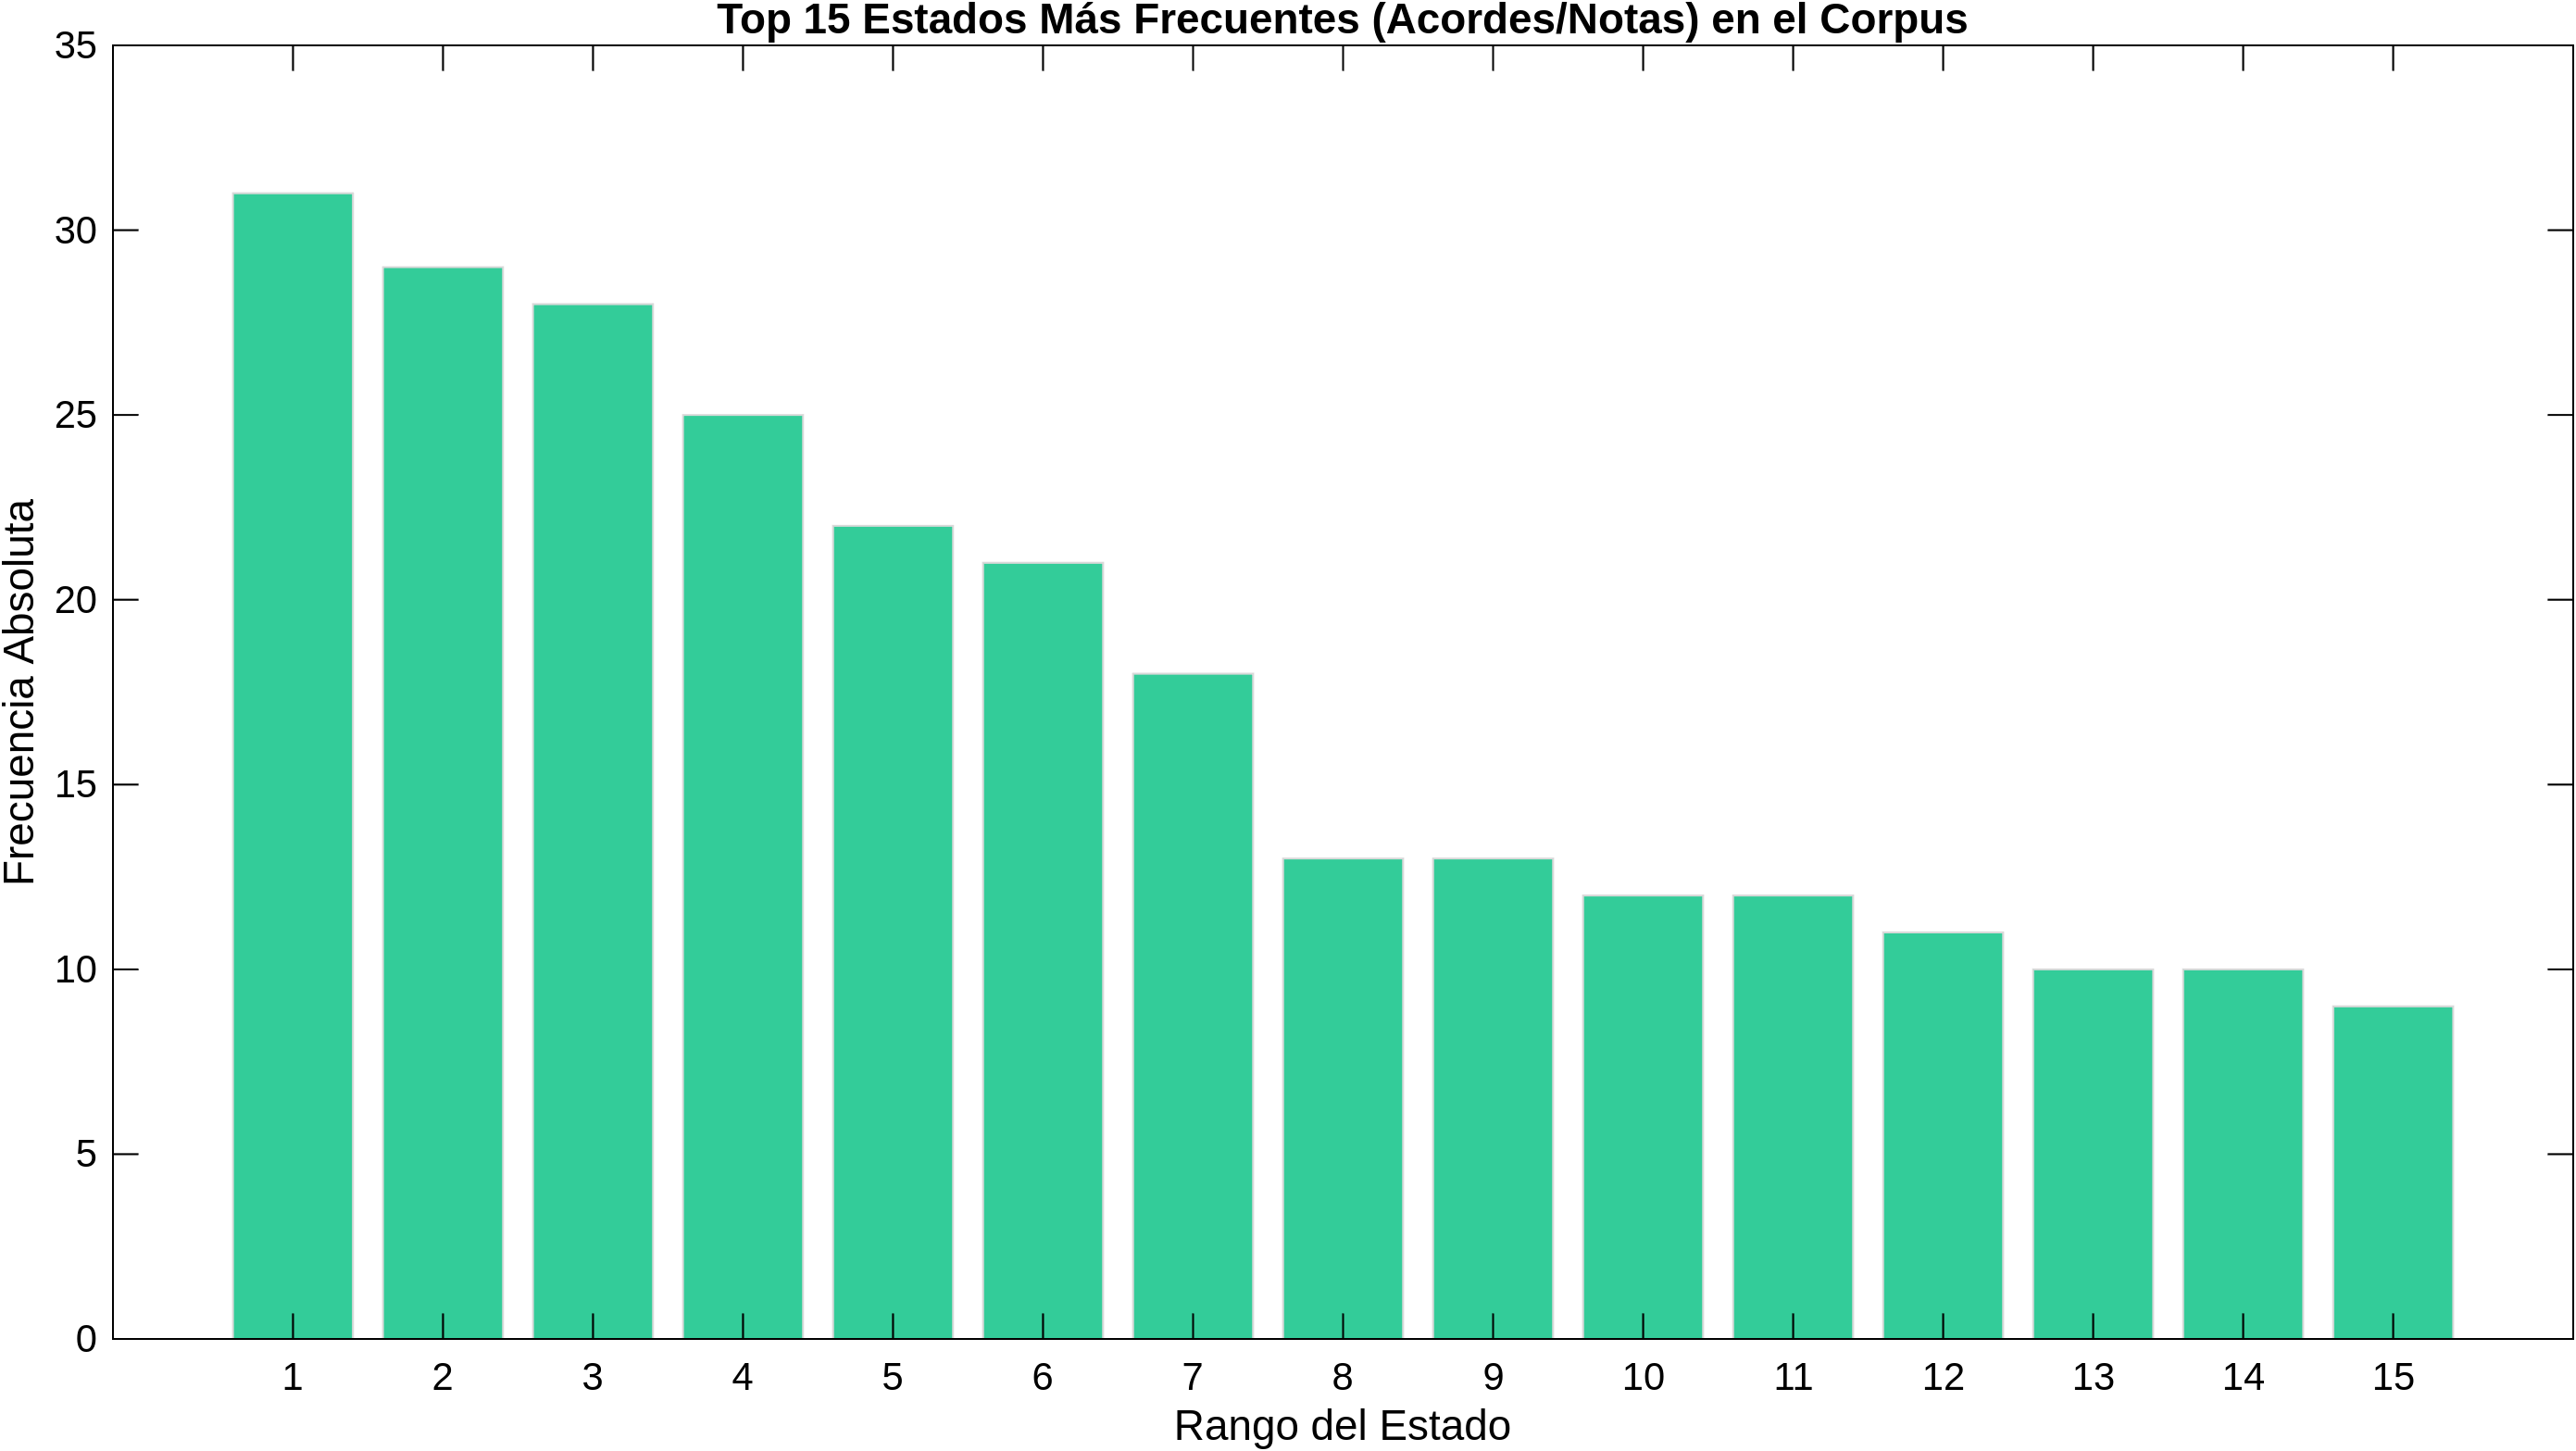
\includegraphics[width=0.8\linewidth]{images/imagenes/actividad7/act7_6_top_estados.png}
	\caption{Distribución de los 15 estados (acordes/notas completas) más frecuentes extraídos del corpus. Estos estados actúan como nodos primarios en el proceso de generación markoviano.}
	\label{fig:act7_top_estados}
\end{figure}

\begin{figure}[H]
	\centering
	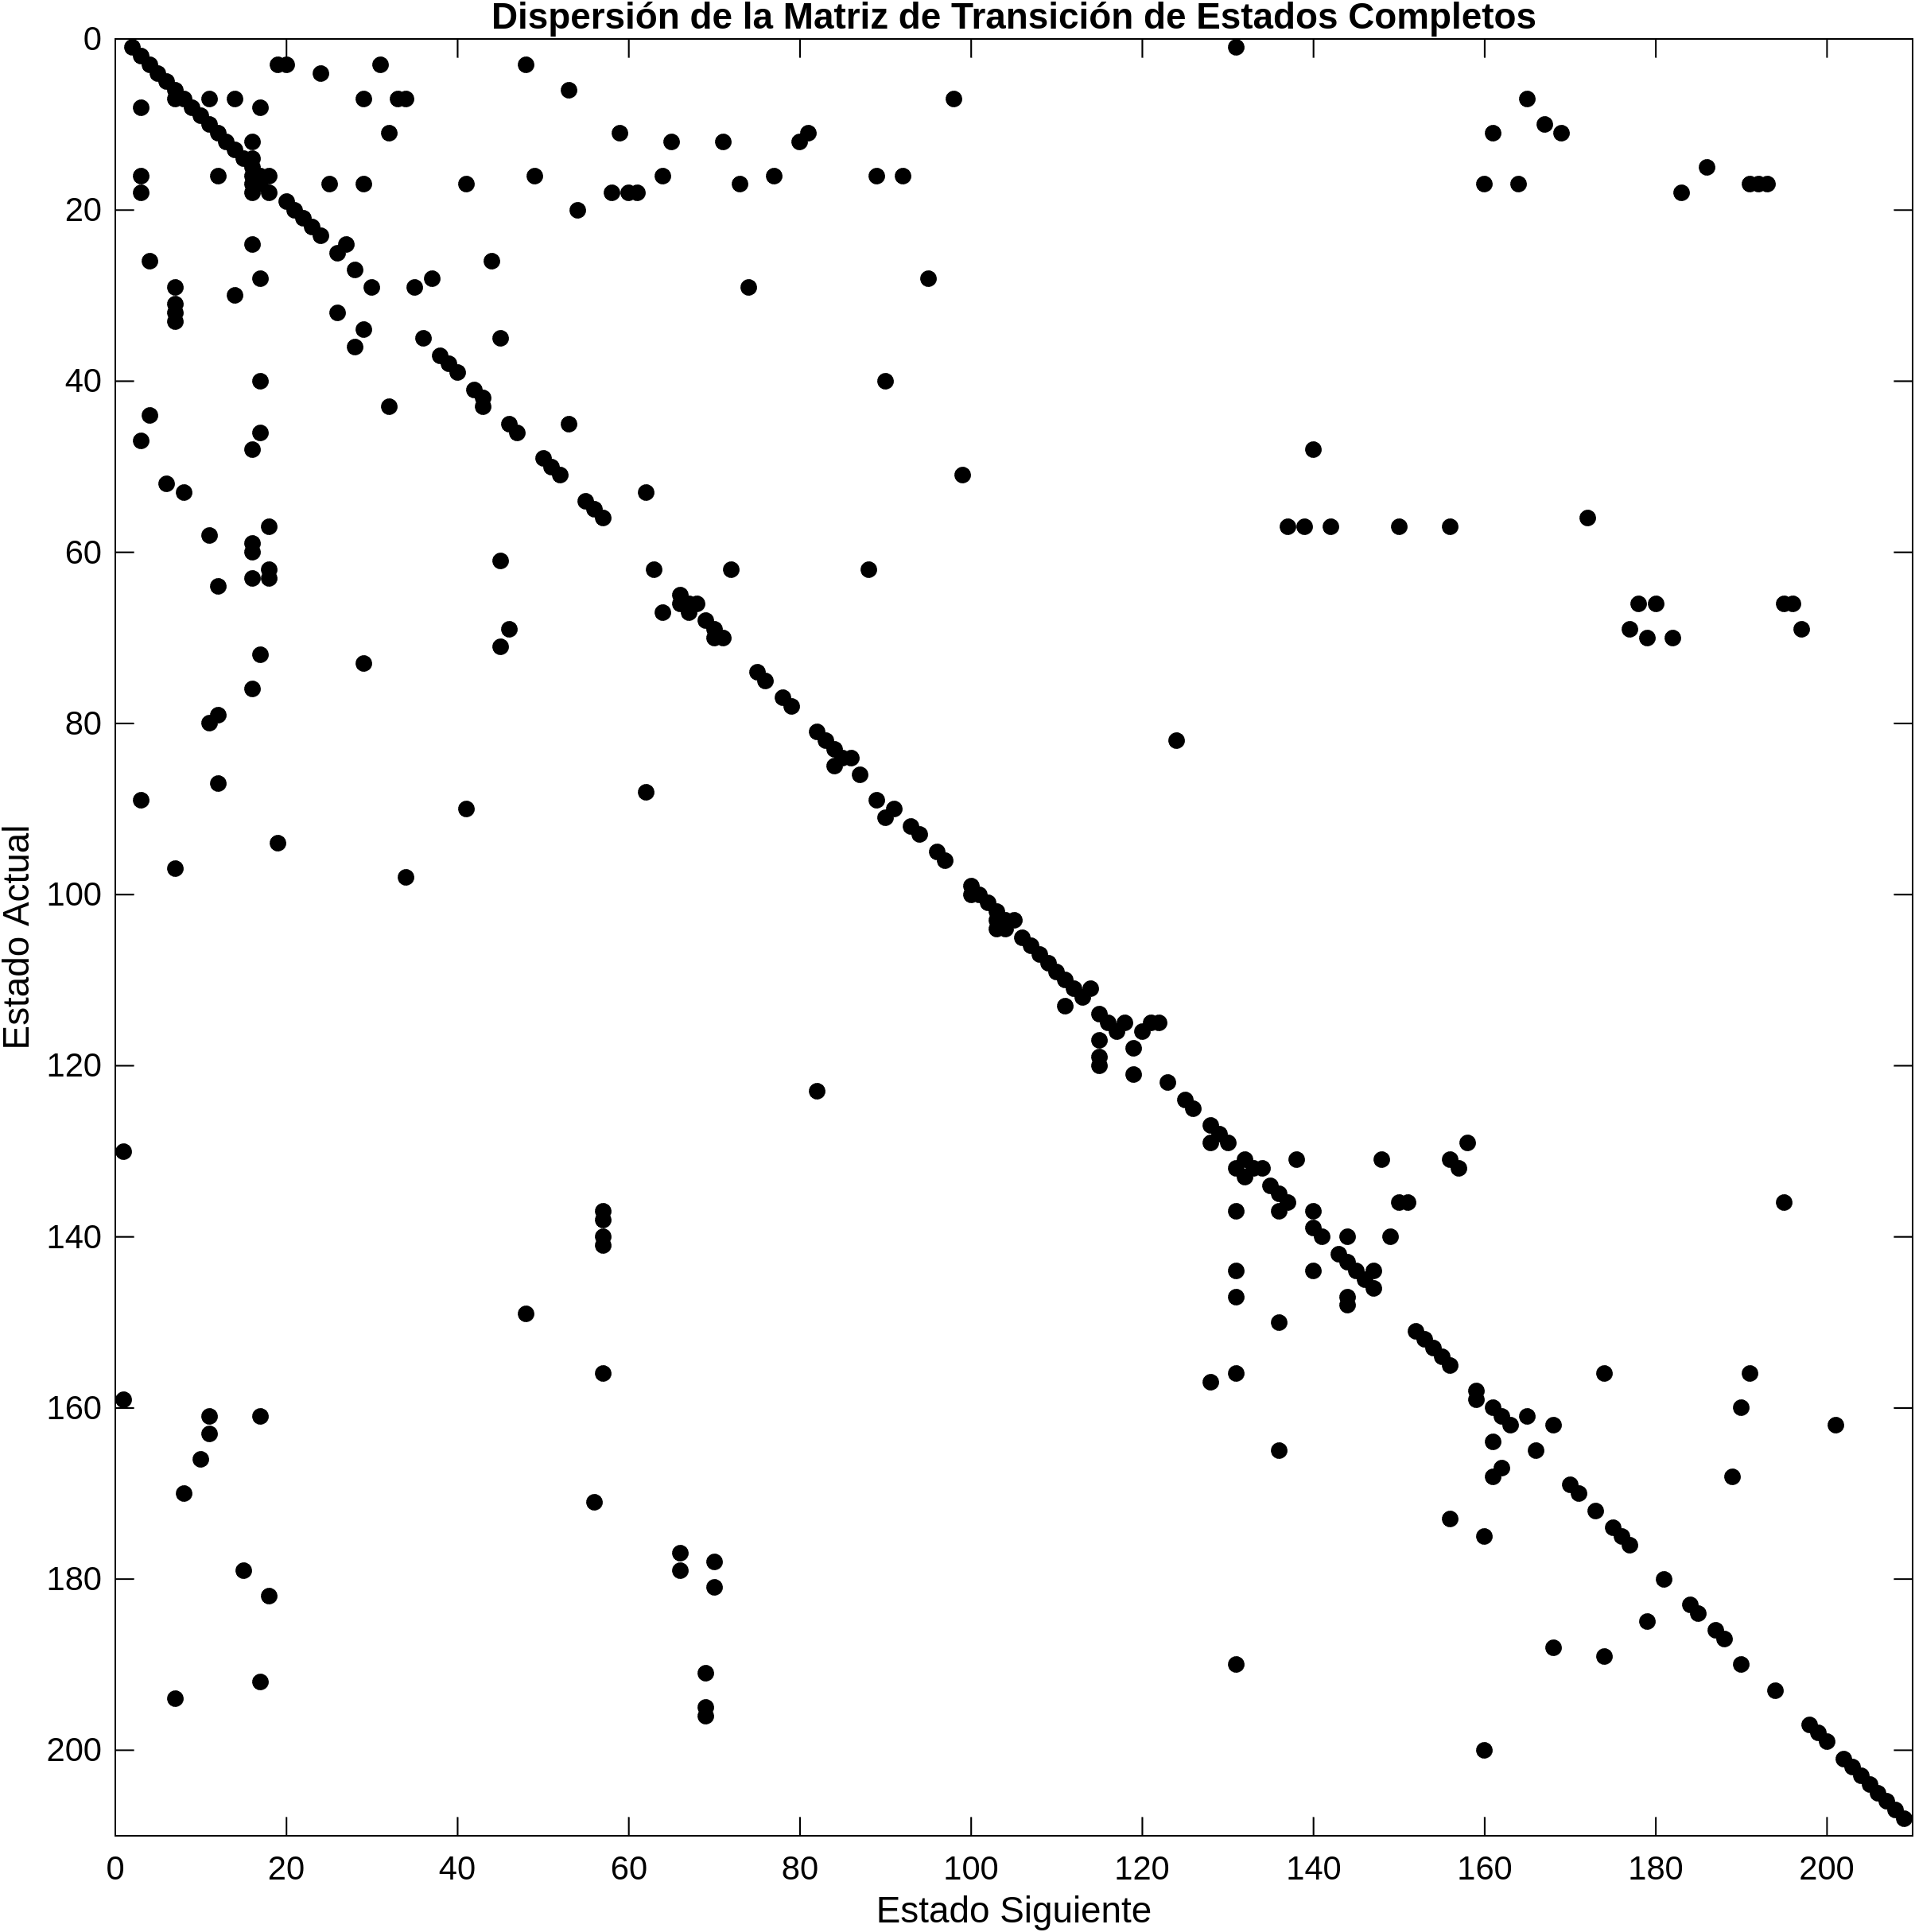
\includegraphics[width=0.6\linewidth]{images/imagenes/actividad7/act7_2_sparsidad_estados.png}
	\caption{Dispersión de la Matriz de Transición de Estados Completos ($209 \times 209$). La alta cantidad de espacio en blanco (ceros) demuestra que las progresiones armónicas no son aleatorias, sino que siguen trayectorias sumamente restringidas y lógicas dictadas por el estilo musical original.}
	\label{fig:act7_sparsidad}
\end{figure}

\begin{figure}[H]
	\centering
	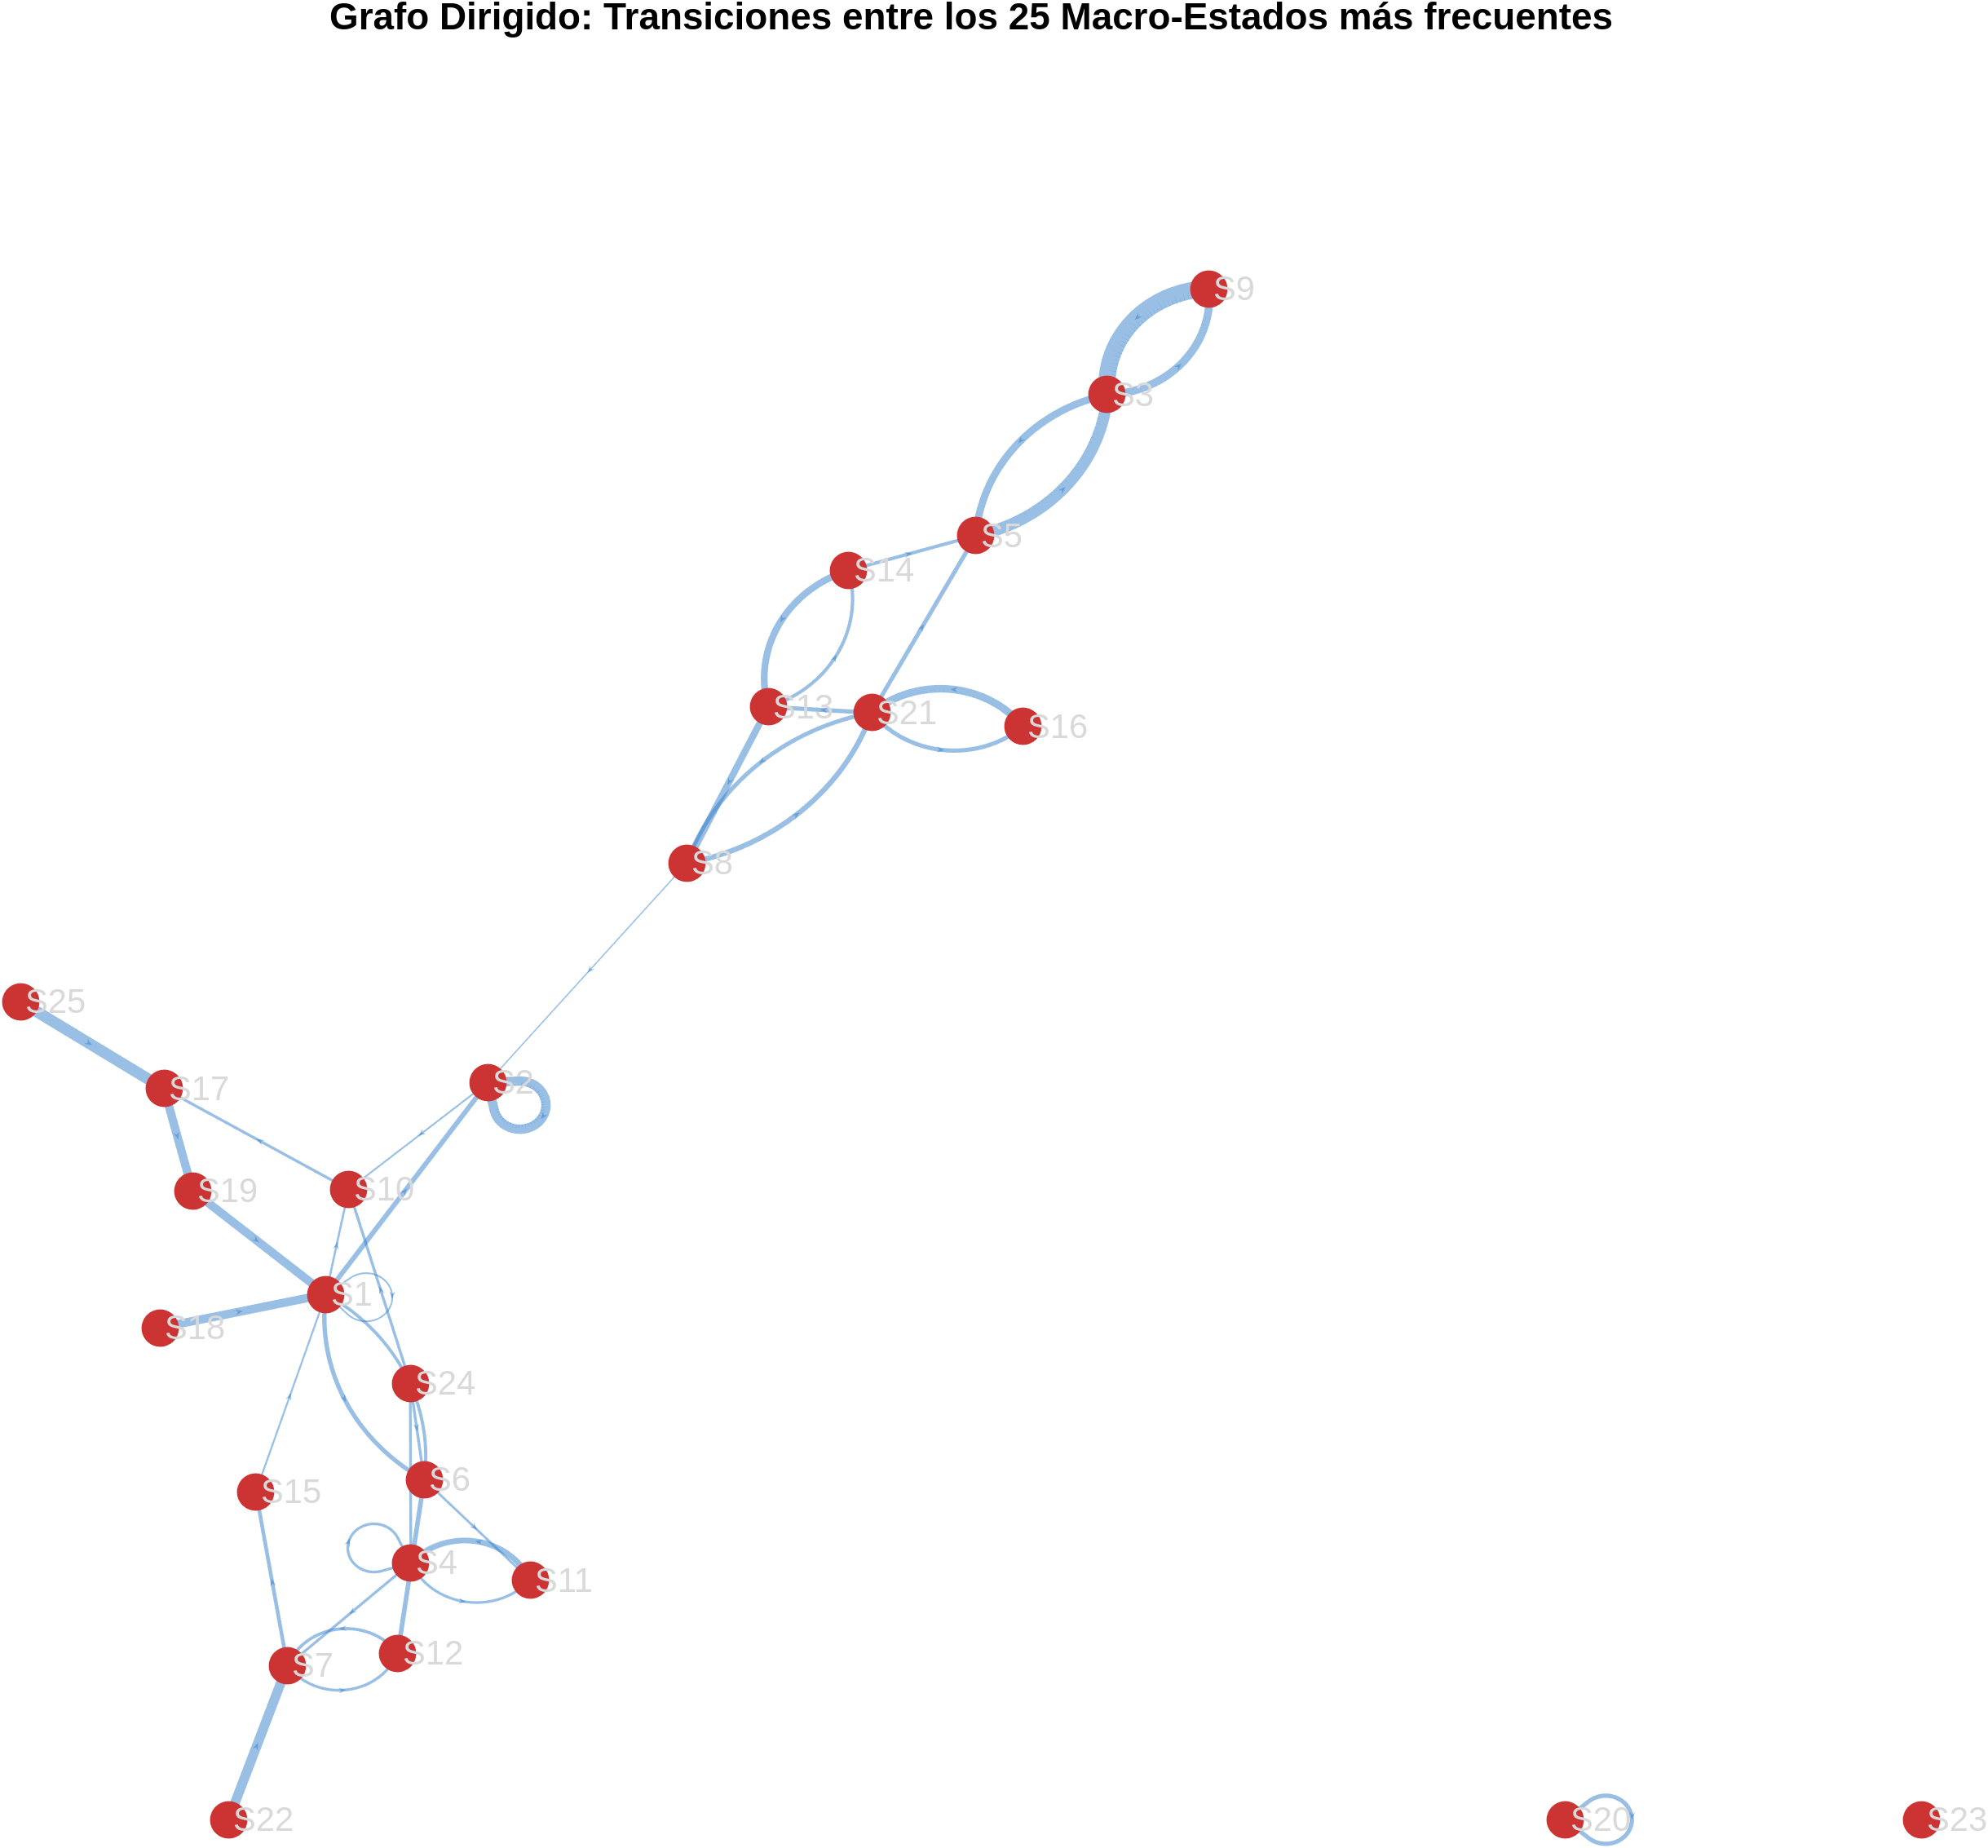
\includegraphics[width=0.8\linewidth]{images/imagenes/actividad7/act7_8_grafo_estados.png}
	\caption{Sub-grafo dirigido de red que ilustra las probabilidades de transición entre los 25 macro-estados más frecuentes ($P > 0.05$). Las aristas más gruesas indican caminos fuertemente predecibles de conducción de voces (resoluciones de tensión).}
	\label{fig:act7_grafo_estados}
\end{figure}

\subsection*{Resultados}
Como resultado del algoritmo, se obtuvo una pieza musical nueva conformada por 200 notas.

Analizando la matriz de transición resultante, se evidenció que es altamente dispersa (posee muchos ceros). Esto indica que el modelo no genera ruido descontrolado, sino que restringe fuertemente las progresiones inválidas y prioriza caminos musicales lógicos. Cualitativamente, al escuchar la salida, la melodía conserva las progresiones de acordes y la coherencia rítmica local de las canciones originales, evidenciando una excelente capacidad de generalización estocástica sin llegar a ser una copia exacta de la obra original.

\section*{Conclusiones}

El desarrollo de este proyecto permite inferir que la música, desde una perspectiva estrictamente probabilística, no puede modelarse como una secuencia de variables aleatorias independientes, debido a que su sintaxis (rítmica y armónica) depende vitalmente de la memoria local del sistema. La notable mejora cualitativa lograda al evolucionar de un modelo de independencia estocástica (Orden 0) a una Cadena de Markov condicional (Orden 1) demuestra empíricamente que la coherencia estética reside en las \textit{probabilidades de transición} y no en las frecuencias absolutas de los eventos aislados. Asimismo, se concluye que tratar el tiempo y la altura (cuerdas/trastes) como procesos estocásticos desvinculados genera disonancias estructurales; la verdadera identidad de un estilo musical sólo emerge cuando ambas dimensiones se entrelazan como un \textit{estado conjunto}, capturando la dependencia multidimensional subyacente.

A partir de estos hallazgos, se propone la aplicación directa de estos modelos matriciales en el diseño de sistemas de audio procesal (generación procedural) para videojuegos, instalaciones artísticas y entornos de realidad virtual. Una matriz de transición de estados completos, finamente extraída de un corpus específico, actúa como un ``motor de improvisación'' capaz de sintetizar atmósferas musicales infinitas y dinámicas que responden al entorno, sin el costo de memoria de almacenar pistas pregrabadas. Por otro lado, desde la perspectiva analítica, las métricas de dependencia cruzada y los grafos dirigidos obtenidos tienen un alto potencial en la musicología computacional, sirviendo como una ``huella dactilar'' biométrica para algoritmos de clasificación de géneros, detección de plagio o verificación de autoría histórica.

Como línea de trabajo futuro, es imprescindible superar las limitaciones inherentes a la propiedad de pérdida de memoria de las Cadenas de Markov de primer orden. Al carecer de contexto histórico profundo, el modelo actual realiza una ``caminata aleatoria'' coherente a corto plazo, pero es incapaz de estructurar formas musicales macro (como estrofa, puente y estribillo). Se proyecta escalar esta arquitectura incorporando Cadenas de Markov de orden superior ($n$-gramas) para encapsular motivos melódicos completos. Finalmente, se sugiere la integración de Modelos Ocultos de Markov (HMM) para desacoplar la progresión armónica (estados latentes) de la ejecución melódica (emisiones observables), sumando también parámetros interpretativos como la intensidad (velocity) y las variaciones sutiles de tempo (rubato) para lograr una síntesis de calidad humana.

\begin{thebibliography}{}
    \bibitem{bertsekas}
    Bertsekas, D.\,P., \& Tsitsiklis, J.\,N. \textit{Introduction to Probability} (2nd\,ed.). Athena Scientific, 2008.

    \bibitem{walpole}
    Walpole, R.\,E., Myers, R.\,H., \& Myers, S.\,L. \textit{Probabilidad y estadística para ingeniería y ciencias} (9a.\,ed.). Pearson Educación, 2012.

    \bibitem{nierhaus2009}
    Nierhaus, G. \textit{Algorithmic Composition: Paradigms of Automated Music Generation}. Springer Science \& Business Media, 2009.

    \bibitem{markov_music}
    Ames, C. \textit{The Markov Process as a Compositional Model: A Survey and Tutorial}. Leonardo, vol. 22, no. 2, 1989, pp. 175-187.

    \bibitem{cope1996}
    Cope, D. \textit{Experiments in Musical Intelligence},A-R Editions, Inc.,1996. 

\end{thebibliography}

\end{document}